% ------------------------------------
\chapter{The adjoint problem}
% ------------------------------------
This chapter is mainly based on the dissertation of Daniel Köhn (\cite{koehn:11}), who originally has written this manual.\\
\newline
The aim of full waveform tomography is to find an ''optimum'' model which can explain the data very well. It should not only explain the 
first arrivals of specific phases of the seismic wavefield like refractions or reflections, but also the amplitudes which contain information 
on the distribution of the elastic material parameters in the underground. To achieve this goal three problems have to be solved:
\begin{enumerate}
\item What is an ''optimum'' model ?
\item How can this model be found ?
\item Is this model unique or are other models existing, which could explain the data equally well ?   
\end{enumerate}
\section{What is an ''optimum'' model ?}
In reflection seismics the $\rm{i^{th}}$ component of the elastic displacement field $\rm{u_i(\mathbf{x_s},\mathbf{x_r},t)}$ 
excited by sources located at $\rm{\mathbf{x_s}}$ will be recorded by receivers at $\rm{\mathbf{x_r}}$ at time t. 
For a given distribution of the material parameters the forward problem Eq. \ref{2:20} can be solved by finite differences (section \ref{elastic_FD_Code}). The result is a model data set $\rm{\mathbf{u^{mod}}}$. This modelled data can be compared with the field data $\rm{\mathbf{u^{obs}}}$. If the misfit or data residuals $\rm{\delta \mathbf{u} = \mathbf{u^{mod}} - \mathbf{u^{obs}}}$ (\FIG{sketch_data_res}) between the modelled and the field data is small the model can explain the data very well. If the residuals are large the model cannot explain the data. The misfit can be measured by a vector norm $\rm{|L|_p}$ which is defined for $\rm{p=1,2,...}$ as  
\begin{equation} 
\rm{|L|_p = \biggl(\sum_i|\delta u_i|^p\biggr)^{1/p}} 
\end{equation} 
The special case $\rm{|L|_\infty}$ is defined as
\begin{equation} 
\rm{|L|_\infty = max_i|\delta u_i|^p} 
\label{l-infty}
\end{equation} 
The L2-norm 
\begin{equation} 
\rm{E=|L|_2 = \frac{1}{2}\mathbf{\delta u^T} \mathbf{\delta u}} 
\label{l-norm}
\end{equation} 
has a special physical meaning. It represents the residual elastic energy contained in the data residuals $\rm{\delta \mathbf{u}}$. An optimum model can be found in a minimum of the residual energy. Therefore the optimum model is the solution of a nonlinear optimization problem.
\begin{figure}[!bh]
\begin{center}
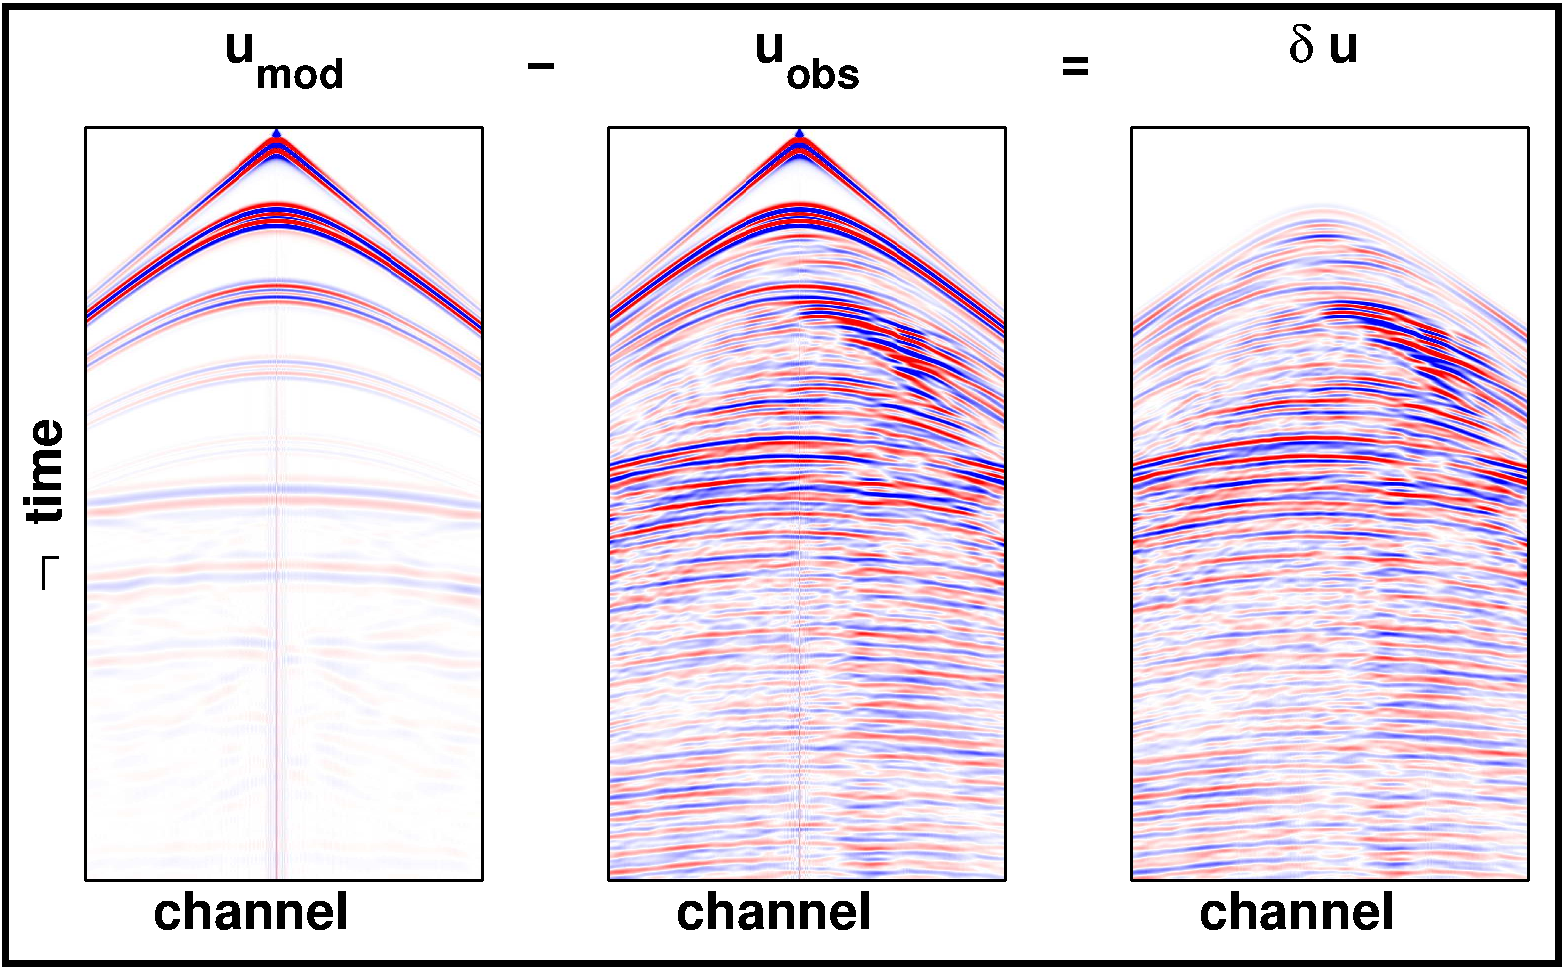
\includegraphics[width=15 cm]{figures/data_res_sketch_1.pdf}
\caption{Definition of data residuals $\rm{\mathbf{\delta u}}$. (\cite{koehn:11})}
\label{sketch_data_res}
\end{center}
\end{figure} 
\newpage
\section{How to find an optimum model}
Figure \ref{sketch_grad} shows a schematic sketch of the residual energy at one point in space as a function of two model parameters 
$\rm{\lambda}$ and $\rm{\mu}$. The colors represent different values of the residual energy. Red areas represent models with high residual 
energy which do not fit the data, while the blue parts are good fitting models with low residual energies. The aim is to find the minimum of 
the residual energy marked by the red cross. Starting at a point $\rm{\mathbf{m_1} = (\lambda_1 (\mathbf{x}), \mu_1 (\mathbf{x}), \rho_1 (\mathbf{x}),)}$ in the parameter space we want to find the minimum by updating the material parameters in an iterative way
\begin{equation} 
\rm{\mathbf{m}_{2} = \mathbf{m}_{1} + \mu_1 \mathbf{\delta m}_{1}, }
\label{eq_update}
\end{equation}
along the search direction $\rm{\mathbf{\delta m}_{1}}$ with the step length $\rm{\mu_1}$. 
\begin{figure}[!bh]
\begin{center}
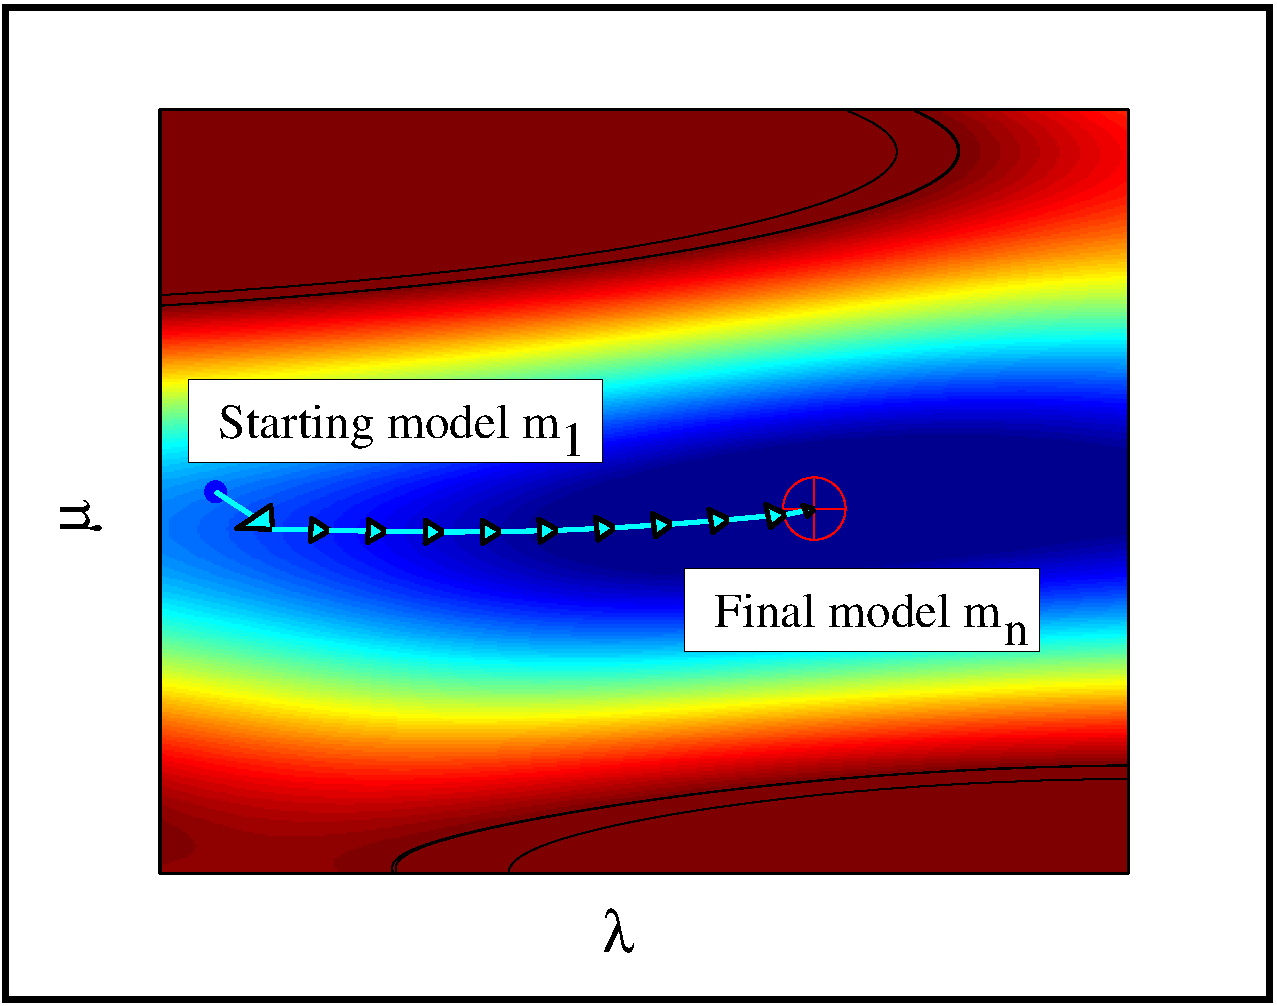
\includegraphics[width=12.5cm]{figures/sketch_grad_1.pdf}
\caption{Schematic sketch of the residual energy at one point in space as a function of two model parameters $\rm{m_1}$ and $\rm{m_2}$. The blue dot denotes the starting point in the parameter space, while the red cross marks a minimum of the objective function. (\cite{koehn:11})}
\label{sketch_grad}
\end{center}
\end{figure} 
To find the optimum search direction $\rm{\mathbf{\delta m}_{1}}$ we expand the residual energy $\rm{E(\mathbf{m}_{1} + \mathbf{\delta m}_{1})}$ near the starting point in a Taylor series:
\begin{equation}
\rm{E(\mathbf{m}_{1} + \mathbf{\delta m}_{1}) \approx E(\mathbf{m}_{1}) + \mathbf{\delta m}_{1} \biggl(\frac{\partial E}{\partial m}\biggr)_1 + \frac{1}{2} \mathbf{\delta m}_{1} \biggl(\frac{\partial^2 E}{\partial m^2}\biggr)_1 \mathbf{\delta m}_{1}^T}   
\label{eq_update_taylor}
\end{equation} 
and set the derivative of Eq. \ref{eq_update_taylor} with respect to $\rm{\delta \mathbf{m_1}}$ zero
\begin{equation}
\rm{\frac{\partial E(\mathbf{m}_{1} + \mathbf{\delta m}_{1})}{\partial \mathbf{\delta m}_{1}} = \biggl(\frac{\partial E}{\partial m}\biggr)_1 + \mathbf{\delta m}_{1} \biggl(\frac{\partial^2 E}{\partial m^2}\biggr)_1 = 0}   
\label{eq_update_taylor_prime}
\end{equation} 
Which finally leads to
\begin{equation}
\rm{\mathbf{\delta m}_{1} = - \biggl(\frac{\partial^2 E}{\partial m^2}\biggr)_1^{-1} \biggl(\frac{\partial E}{\partial m}\biggr)_1 = -  \mathbf{H_1}^{-1} \biggl(\frac{\partial E}{\partial m}\biggr)_1}   
\label{eq_opt_search}
\end{equation} 
where $\rm{(\partial E/\partial \mathbf{m})_1}$ denotes the steepest-descent direction of the objective function and $\rm{\mathbf{H_1}^{-1}}$ the inverse Hessian matrix. The inverse Hessian matrix for the elastic problem is often singular and can only be calculated with high computational costs. Therefore the inverse Hessian matrix is approximated by a preconditioning operator P. There is no general rule for an optimum preconditioning operator. 
\begin{equation}
\rm{\mathbf{\delta m}_{1} \approx - \mathbf{P_1} \biggl(\frac{\partial E}{\partial m}\biggr)_1.}   
\label{eq_opt_search1}
\end{equation} 
By replacing $\rm{\mathbf{\delta m}_{1}}$ in Eq. \ref{eq_update} with Eq. \ref{eq_opt_search1} we get         
\begin{equation} 
\rm{\mathbf{m}_{2} = \mathbf{m}_{1} - \mu_1 \mathbf{P_1} \biggl(\frac{\partial E}{\partial \mathbf{m}}\biggr)_1, }
\label{eq_update1}
\end{equation} 
The optimum model parameters can be found along the negative gradient direction of the residual energy. The starting point $\rm{\mathbf{m_1}}$ is not a particular point, so the update function can be applied to every point in the parameter space $\rm{\mathbf{m_n}}$ 
\begin{equation} 
\rm{\mathbf{m}_{n+1} = \mathbf{m}_{n} - \mu_n \mathbf{P_n} \biggl(\frac{\partial E}{\partial \mathbf{m}}\biggr)_n. }
\label{eq_updatefinal}
\end{equation} 

\section{Calculation of the gradient direction}% $\rm{\frac{\partial E}{\partial \mathbf{m}}}$}
To estimate the gradient direction $\rm{\partial E/\partial \mathbf{m}}$ the residual energy is rewritten as:
\begin{equation} 
\rm{E = \frac{1}{2}\mathbf{\delta u^T} \mathbf{\delta u} = \frac{1}{2} \sum_{sources} \int dt \sum_{receiver} \mathbf{\delta u}^2(x_r, x_s, t) } 
\label{L2_continous}
\end{equation}
After derivation with respect to a model parameter $\rm{\mathbf{m}}$ we get
\begin{equation} 
\begin{split}
\rm{\frac{\partial E}{\partial \mathbf{m}}} &\rm{= \sum_{sources} \int dt \sum_{receiver} \frac{\partial \mathbf{\delta u}}{\partial
\mathbf{m}} \mathbf{\delta u}}\\ 
& \rm{= \sum_{sources} \int dt \sum_{receiver} \frac{\partial {(\mathbf{u^{mod}\mathbf(m)} - \mathbf{u^{obs}})}}{\partial
\mathbf{m}}  \mathbf{\delta u} }\\ 
&\rm{= \sum_{sources} \int dt \sum_{receiver} \frac{\partial {\mathbf{u^{mod}(\mathbf{m})}}}{\partial \mathbf{m}}  \mathbf{\delta u}} 
\label{dL2_dm}
\end{split}
\end{equation}
Eq. \ER{dL2_dm} can be related to the mapping of small changes from the data to the model space and vice versa (\FIG{mapping_data_model}). 
\begin{figure}[ht]
\begin{center}
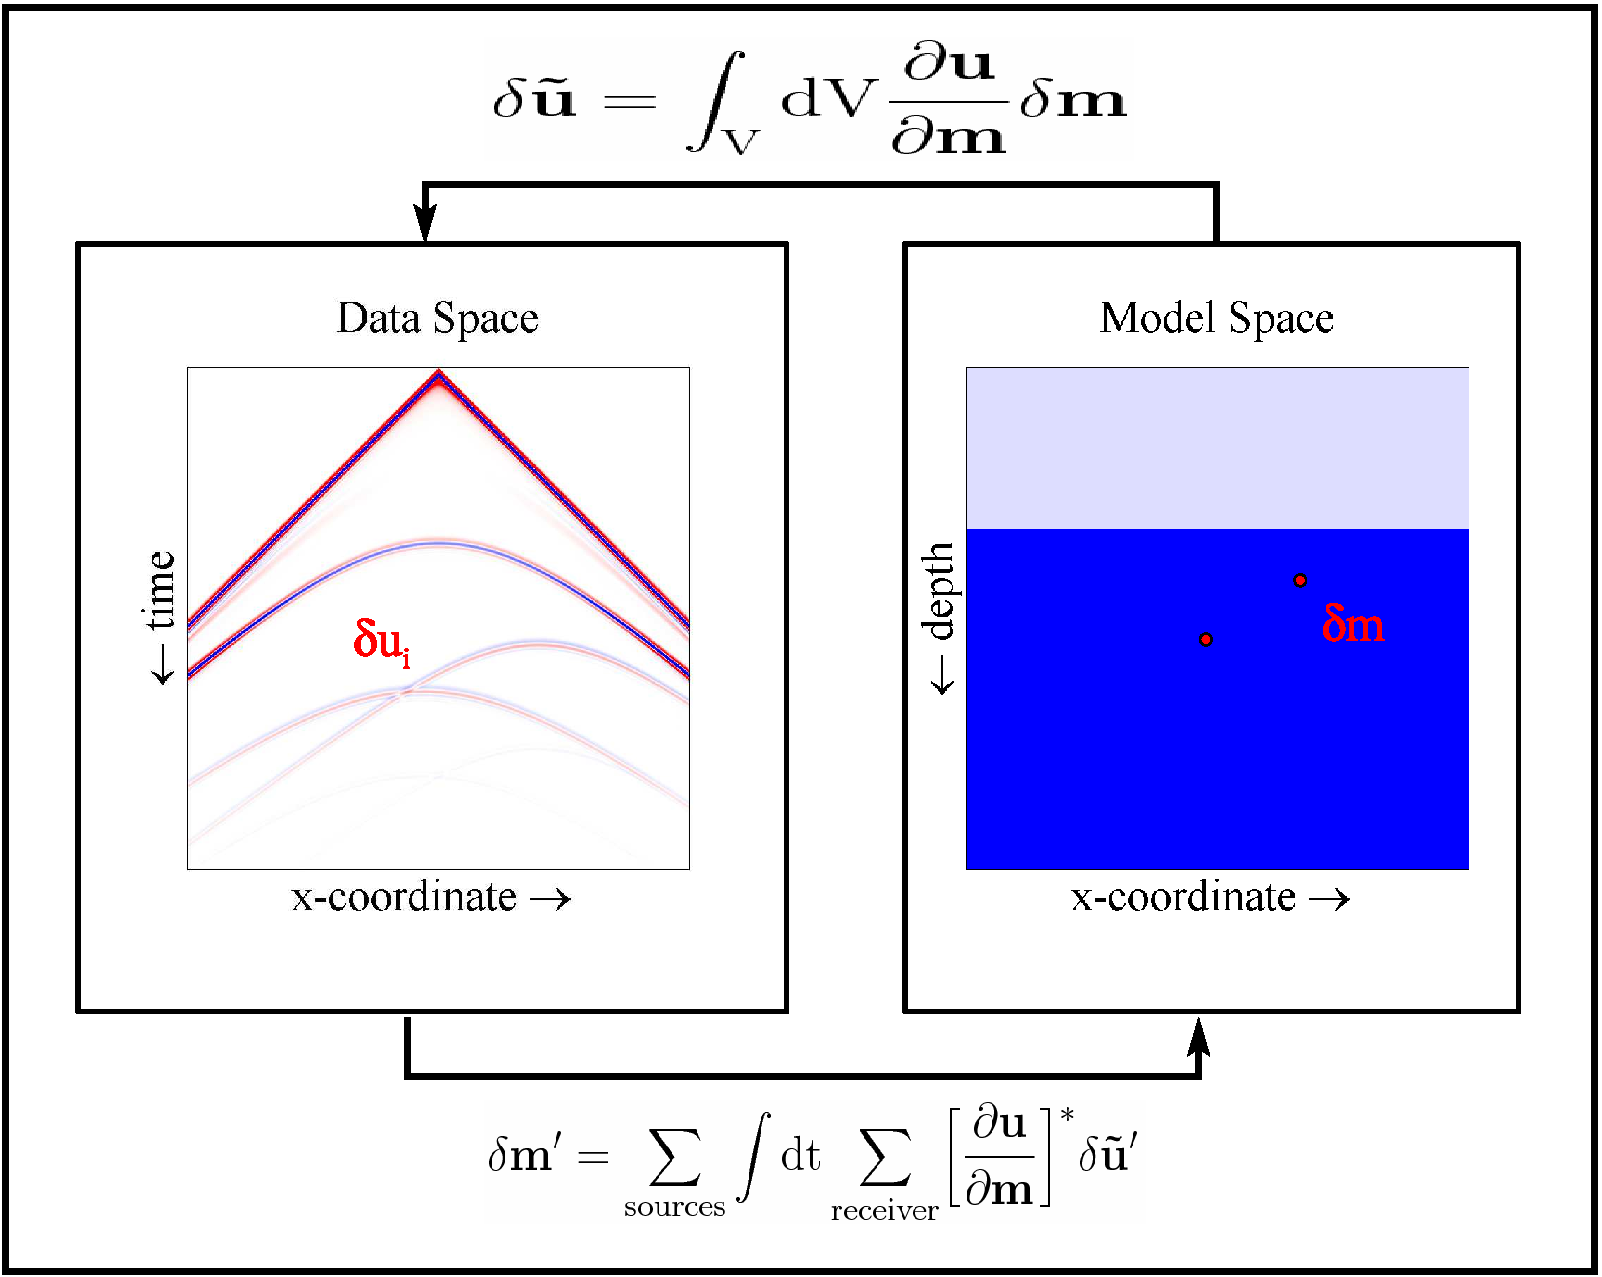
\includegraphics[width=10cm]{figures/mapping_data_model.pdf}
\caption{Mapping between model and data space and vice versa. (\cite{koehn:11})}
\label{mapping_data_model}
\end{center}
\end{figure}
A small change in the model space $\rm{\delta \mathbf{m}}$, e.g. one model parameter at one point in space, will result in a small 
perturbation of the data space $\rm{\delta \mathbf{\tilde{u}}}$, e.g. one wiggle in the seismic section. If the Frech$\rm{\acute{e}}$t derivative $\rm{\frac{\partial \mathbf{u}}{\partial \mathbf{m}}}$ is known, all 
the small perturbations in model space can be integrated over the model volume V to calculate the total change in data space
(\cite{tarantola:2005}):
\begin{equation}
\rm{\delta \mathbf{\tilde{u}}(\mathbf{x_s},\mathbf{x_r},t) = \int_V dV \frac{\partial \mathbf{u}}{\partial \mathbf{m}} \delta 
\mathbf{m},}
\label{2:4}
\end{equation} 
or by introducing the linear operator $\rm{\hat{L}}$
\begin{equation}
\rm{\delta \mathbf{\tilde{u}} = \hat{L} \delta \mathbf{m} := \int_V dV \frac{\partial \mathbf{u}}{\partial \mathbf{m}} \delta 
\mathbf{m}.\notag}
\label{2:4:1}
\end{equation} 
In a similar way small changes in the data space $\rm{\delta \mathbf{\tilde{u}}'}$ can be integrated to calculate the total change in the model 
space $\rm{\delta \mathbf{m}'}$ (\cite{tarantola:2005})
\begin{equation}
\rm{\delta \mathbf{m'} =  \sum_{sources} \int dt \sum_{receiver} \biggl[\frac{\partial \mathbf{u}}{\partial \mathbf{m}}\biggr]^* \delta
\mathbf{\tilde{u}}',}
\label{3:6}
\end{equation}
or as operator equation
\begin{equation}
\rm{\delta \mathbf{m'} = \hat{L}^* \delta \mathbf{\tilde{u}}'. \notag}
\label{3:6:1}
\end{equation}
In this case the Frech$\rm{\acute{e}}$t derivative $\rm{\frac{\partial \mathbf{u}}{\partial \mathbf{m}}}$ is replaced by it's adjoint 
counterpart $\rm{\frac{\partial \mathbf{u}}{\partial \mathbf{m}}^*}$. Note that $\rm{\delta
\mathbf{\tilde{u}} \ne \delta \mathbf{\tilde{u}}'}$ and $\rm{\delta \mathbf{m} \ne \delta \mathbf{m}'}$, so there is no unique way to map perturbations from the model to the data space or vice versa. Because the operator $\rm{\hat{L}}$ is linear, the kernel of $\rm{\hat{L}}$ and it's adjoint counterpart $\rm{\hat{L}^*}$ are identical (see chapter 5.4.2 in \cite{tarantola:2005})
\begin{equation}
\rm{\biggl[\frac{\partial \mathbf{u}}{\partial \mathbf{m}}\biggr]^* = \biggl[\frac{\partial \mathbf{u}}{\partial \mathbf{m}}\biggr]} \notag
\end{equation}
Therefore the mapping from the data to the model space Eq. \ER{3:6} is equal to the gradient of the residual energy Eq. \ER{dL2_dm}: 

\begin{equation}
\begin{split}
\rm{\delta \mathbf{m'}} &\rm{=  \sum_{sources} \int dt \sum_{receiver} \biggl[\frac{\partial \mathbf{u_i}}{\partial \mathbf{m}}\biggr]^*
\delta \mathbf{\tilde{u}}'} \\
                   &\rm{=  \sum_{sources} \int dt \sum_{receiver} \biggl[\frac{\partial \mathbf{u_i}}{\partial \mathbf{m}}\biggr] \delta \mathbf{u}} \\
                   &\rm{=  \frac{\partial E}{\partial \mathbf{m}}}
\end{split}
\label{dm_dE_dm}
\end{equation}
if the perturbation of the data space $\rm{\delta \mathbf{\tilde{u}}'}$ is interpretated as data residuals $\rm{\delta \mathbf{u}}$. So the approach to estimate the gradient direction $\rm{\partial E/\partial m}$ can be split into 3 parts
\begin{enumerate}
\item Find a solution to the forward problem
\begin{equation}
\rm{\delta \mathbf{u} = \hat{L} \delta \mathbf{m}.\notag}
\end{equation} 
\item Identify the Frech$\rm{\acute{e}}$t kernels $\rm{\partial \mathbf{u}/\partial \mathbf{m}}$ 
\item Use the property, that a linear operator $\rm{\hat{L}}$ and it's adjoint $\rm{\hat{L}^*}$ have the same kernels and calculate the gradient direction by using:
\begin{equation}
\rm{\frac{\partial E}{\partial \mathbf{m}} = \delta \mathbf{m'} = \hat{L}^* \delta \mathbf{u}'. \notag}
\end{equation} 
\end{enumerate}
This is a very general approach. Now we apply this approach to the equations of motion for an elastic medium. The following derivation is much easier, when assuming a general elastic medium first and introduce the isotropy later on. Therefore the elastic forward problem Eqs. \ER{2:20} can be written as 
\begin{equation}
\begin{split}
\rm{\rho} & \rm{\frac{\partial^2 u_i}{\partial t^2} - \frac{\partial}{\partial x_j} \sigma_{ij}} \rm{=f_i,} \\
\rm{\sigma_{ij}} & \rm{- c_{ijkl} \epsilon_{kl}} \rm{= T_{ij},}\\
\rm{\epsilon_{ij}} &\rm{= \frac{1}{2} \biggl(\frac{\partial u_i}{\partial x_j}+\frac{\partial u_j}{\partial x_i}\biggr),}\\
&\rm{\text{+ initial and boundary conditions},}\\
\label{2:1}
\end{split}
\end{equation}
where $\rm{\rho}$ denotes the density, $\rm{\sigma_{ij}}$ the stress tensor, $\rm{\epsilon_{ij}}$ the strain tensor, $c_{ijkl}$ the stiffness tensor, $\rm{f_i}$, $\rm{T_{ij}}$ source terms for volume and surface forces, respectively. 
In the next step every parameter and variable in the elastic wave equation is perturbated by a first order perturbation as shown in Fig. \ref{mapping_data_model}:
\begin{equation}
\begin{split}
\rm{u_i} & \rm{\rightarrow u_i + \delta u_i,}\\
\rm{\rho} & \rm{\rightarrow \rho + \delta \rho,}\\
\rm{\sigma_{ij}} & \rm{\rightarrow \sigma_{ij} + \delta \sigma_{ij},}\\
\rm{c_{ijkl}} & \rm{\rightarrow c_{ijkl} + \delta c_{ijkl},}\\
\rm{\epsilon_{ij}} & \rm{\rightarrow \epsilon_{ij} + \delta \epsilon_{ij},}\\
\end{split}
\label{2:10}
\end{equation}
These substitutions yield new equations of motion describing the displacement perturbations $\rm{\delta u_i}$ and stress perturbations $\rm{\delta \sigma_{ij}}$ as a function of new source 
terms $\rm{\Delta f_i}$ and $\rm{\Delta T_{ij}}$      
\begin{equation}
\begin{split}
\rm{\rho} & \rm{ \frac{\partial^2 \delta u_i}{\partial t^2} - \frac{\partial}{\partial x_j} \delta \sigma_{ij}} \rm{= \Delta f_i,} \\
\rm{\delta \sigma_{ij}} & \rm{- c_{ijkl} \delta \epsilon_{kl}} \rm{= \Delta T_{ij},}\\
\rm{\delta \epsilon_{ij}} &\rm{= \frac{1}{2} \biggl(\frac{\partial \delta u_i}{\partial x_j}+\frac{\partial \delta u_j}{\partial
x_i}\biggr)}\\
& \rm{\text{+ perturbated initial and boundary conditions}} \\
\end{split}
\label{2:11}
\end{equation}
The new source terms are 
\begin{equation}
\begin{split}
\rm{\Delta f_i} & \rm{= - \delta \rho \frac{\partial^2 u_i}{\partial t^2}}
\end{split}
\label{2:12}
\end{equation}
and
\begin{equation}
\begin{split}
\rm{\Delta T_{ij}} & \rm{= \delta c_{ijkl} \epsilon_{kl}.}
\end{split}
\label{2:13}
\end{equation}
Two points are important to notice: 
\begin{enumerate}
\item Eq.(\ref{2:11}) states that every change of a material parameter acts as a source 
(Eq.(\ref{2:12}) and Eq.(\ref{2:13})), but the perturbated wavefield is propagating in the unperturbated medium. 
\item The new wave equation (\ref{2:11}) has mathematically the same form as the unperturbated elastic wave equation, and hence its solution can be obtained in terms of
Green's functions $\rm{G_{ij}}$ of the elastic wave equation. 
\end{enumerate}
The solution of the perturbated elastic equations of motion \ER{2:11} in terms of the elastic Green's function $\rm{G_{ij}(\mathbf{x},t;\mathbf{x'},t')}$ can be written as: 
\begin{equation}
\begin{split}
\rm{\delta u_i(\mathbf{x},t)} & \rm{= \int_V dV \int_0^T dt' G_{ij}(x,t;x',t')\Delta f_j(\mathbf{x'},t')}\\ 
& \rm{- \int_V dV \int_0^T dt' \frac{\partial G_{ij}}{\partial x'_k}(x,t;x',t')\Delta T_{jk}(\mathbf{x'},t').}
\end{split}
\label{2:14}
\end{equation} 

Substituting the force and traction terms given by Eqs.(\ref{2:12}) and (\ref{2:13}) into Eq.(\ref{2:14}) yields after some rearranging
\begin{equation}
\begin{split}
\rm{\delta u_i(\mathbf{x},t)} & \rm{= -\int_V dV \int_0^T dt' G_{ij}(x,t;x',t') \frac{\partial^2 u_j}{\partial t^2}(\mathbf{x'},t') \delta \rho}\\ 
& \rm{- \int_V dV \int_0^T dt' \frac{\partial G_{ij}}{\partial x'_k}(x,t;x',t') \epsilon_{lm}(\mathbf{x'},t') \delta c_{jklm}}
\end{split}
\label{adj2:20}
\end{equation}

Introducing isotropy 
%via Eq. \ER{2:17:1} 
leads to:

\begin{equation}
\begin{split}
\rm{\delta u_i(\mathbf{x},t)} & \rm{= -\int_V dV \biggl[ \int_0^T dt' G_{ij}(x,t;x',t') \frac{\partial^2 u_j}{\partial t^2}(\mathbf{x'},t') \biggr] \delta \rho}\\ 
& \rm{- \int_V dV \biggl[ \int_0^T dt' \frac{\partial G_{ij}}{\partial x'_k}(x,t;x',t') \epsilon_{lm}(\mathbf{x'},t') \delta_{jk} \delta_{lm} \biggr] \delta \lambda}\\
& \rm{- \int_V dV \biggl[ \int_0^T dt' \frac{\partial G_{ij}}{\partial x'_k}(x,t;x',t') \epsilon_{lm}(\mathbf{x'},t') (\delta_{jl} \delta_{lm} + \delta_{jm} \delta_{kl}) \biggr] \delta \mu.}
\end{split}
\label{adj2:20:1}
\end{equation}
Utilization of Eq.(\ref{adj2:20:1}) to solve the forward problem is known as the Born approximation. In waveform tomography the Born approximation is not used to solve the forward problem. 
Instead the full elastic wave equation is solved. Equation \ER{adj2:20:1} has the same form as the desired expression for the forward problem Eqs.(\ref{2:4}):
\begin{equation}
\rm{\delta \mathbf{u} = \int_V dV \frac{\partial \mathbf{u}}{\partial \mathbf{m}} \delta \mathbf{m}.}
\label{adj2:20:1:1}
\end{equation} 
Therefore the Frech$\rm{\acute{e}}$t kernels $\rm{\frac{\partial u_i}{\partial 
\mathbf{m(x)}}}$ for the individual material parameters can be identified as:
\begin{equation}
\begin{split}
\rm{\frac{\partial u_i}{\partial \mathbf{\rho}}} &= \rm{-\int_0^T dt' G_{ij}(x,t;x',t') \frac{\partial^2 u_j}{\partial t^2}(\mathbf{x'},t')} \\
\rm{\frac{\partial u_i}{\partial \mathbf{\lambda}}} &= \rm{-\int_0^T dt' \frac{\partial G_{ij}}{\partial x'_k}(x,t;x',t') \epsilon_{lm}(\mathbf{x'},t') \delta_{jk} \delta_{lm}} \\
\rm{\frac{\partial u_i}{\partial \mathbf{\mu}}} &= \rm{-\int_0^T dt' \frac{\partial G_{ij}}{\partial x'_k}(x,t;x',t') \epsilon_{lm}(\mathbf{x'},t') (\delta_{jl} \delta_{lm} + \delta_{jm} \delta_{kl}) } \\ 
\label{adj2:20:2}
\end{split}
\end{equation}
By definition the adjoint of the operator \ER{adj2:20:1:1} can be written as 
\begin{equation}
\rm{\delta \mathbf{m'(x)} = \sum_{sources} \int_0^T dt \sum_{\rm{\alpha=1}}^{\rm{N_{rec}}} \biggl[\frac{\partial u_i}{\partial
\mathbf{m}} \biggl]^* \delta u_i'(\mathbf{x_\alpha},t'),}
\label{adj2:20:3}
\end{equation}
Because a linear operator and its transpose have the same kernels $\rm{\partial u_i/\partial \mathbf{m}}$, the only difference arise in the variables of sum/integration, which are complementary. Inserting the integral kernels \ER{adj2:20:2} in Eq.\ER{adj2:20:3} yields  
\begin{equation} 
\begin{split}
\rm{\delta \rho'} &\rm{= - \sum_{sources} \int_0^T dt \sum_{\alpha=1}^{\rm{N_{rec}}} \int_0^T dt' G_{ij}(\mathbf{x_\alpha},t';\mathbf{x},t) \frac{\partial^2 u_j}{\partial t^2}(\mathbf{x},t) \delta u_i'(x_\alpha,t'),}\\
\rm{\delta \lambda'} &\rm{= - \sum_{sources} \int_0^T dt \sum_{\alpha=1}^{\rm{N_{rec}}} \int_0^T dt' \frac{\partial G_{ij}}{\partial x_k}(\mathbf{x_\alpha},t';\mathbf{x},t) \epsilon_{lm}(\mathbf{x},t) \delta_{jk} \delta_{lm} \delta u_i'(\mathbf{x_\alpha},t'),}\\
\rm{\delta \mu'} &\rm{= - \sum_{sources} \int_0^T dt \sum_{\alpha=1}^{\rm{N_{rec}}} \int_0^T dt' \frac{\partial G_{ij}}{\partial x_k}(\mathbf{x_\alpha},t';\mathbf{x},t) \epsilon_{lm}(\mathbf{x},t) (\delta_{jl} \delta_{lm} + \delta_{jm} \delta_{kl}) \delta u_i'(\mathbf{x_\alpha},t').} \notag
\end{split} 
\end{equation} 
The terms only depending on time $\rm{t}$ and the positions $\rm{\mathbf{x}}$ can be moved infront of the sum over the receivers
\begin{equation} 
\begin{split}
\rm{\delta \rho'} &\rm{= - \sum_{sources} \int_0^T dt \frac{\partial^2 u_j}{\partial t^2}(\mathbf{x},t) \sum_{\alpha=1}^{\rm{N_{rec}}} \int_0^T dt' G_{ij}(\mathbf{x_\alpha},t';\mathbf{x},t) \delta u_i'(x_\alpha,t'),}\\
\rm{\delta \lambda'} &\rm{= - \sum_{sources} \int_0^T dt \epsilon_{lm}(\mathbf{x},t) \delta_{jk} \delta_{lm} \sum_{\alpha=1}^{\rm{N_{rec}}} \int_0^T dt' \frac{\partial G_{ij}}{\partial x_k}(\mathbf{x_\alpha},t';\mathbf{x},t) \delta u_i'(\mathbf{x_\alpha},t'),}\\
\rm{\delta \mu'} &\rm{= - \sum_{sources} \int_0^T dt \epsilon_{lm}(\mathbf{x},t) (\delta_{jl} \delta_{lm} + \delta_{jm} \delta_{kl}) \sum_{\alpha=1}^{\rm{N_{rec}}} \int_0^T dt' \frac{\partial G_{ij}}{\partial x_k}(\mathbf{x_\alpha},t';\mathbf{x},t) \delta u_i'(\mathbf{x_\alpha},t').}
\end{split} 
\label{A3:10}
\end{equation} 
Defining the wavefield 
\begin{equation} 
\begin{split}
\rm{\Psi_j (\mathbf{x},t)} &\rm{= \sum_{\alpha=1}^{\rm{N_{rec}}} \int_0^T dt' G_{ij}(x_\alpha,t';\mathbf{x},t) \delta u_i'(x_\alpha,t'),}
\end{split} 
\label{A3:20}
\end{equation}
Eqs.\ER{A3:10} can be written as
\begin{equation}
\begin{split} 
\rm{\delta \rho'} &\rm{= - \sum_{sources} \int_0^T dt \frac{\partial^2 u_j}{\partial t^2}(\mathbf{x},t) \Psi_j,}\\
\rm{\delta \lambda'} &\rm{= - \sum_{sources} \int_0^T dt \epsilon_{lm}(\mathbf{x},t) \delta_{jk} \delta_{lm} \frac{\partial \Psi_{j}}{\partial x_k},}\\
\rm{\delta \mu'} &\rm{= - \sum_{sources} \int_0^T dt \epsilon_{lm}(\mathbf{x},t) (\delta_{jl} \delta_{lm} + \delta_{jm} \delta_{kl}) \frac{\partial \Psi_{j}}{\partial x_k}.} 
\label{A3:30:3}
\end{split}
\end{equation} 

The wavefield $\rm{\Psi_j}$ is generated by propagating the residual data $\rm{\delta u_i'}$ from the receiver positions backwards in
time through the elastic medium. 
To obtain a more symmetric expression for the density gradient, let us integrate the density gradient in \ER{A3:30:3} by parts
\begin{equation} 
\begin{split}
\rm{\delta \rho'} &\rm{= - \sum_{sources} \int_0^T dt \biggl(\frac{\partial^2 u_j}{\partial t^2}(\mathbf{x},t)\biggr) \Psi_j (\mathbf{x},t)} \\
&\rm{= - \sum_{sources} \biggl\{\biggl[\frac{\partial u_j}{\partial t}(\mathbf{x},T) \Psi_j (\mathbf{x},T)\biggr]_0^T - \int_0^T dt \frac{\partial u_j}{\partial t}(\mathbf{x},t) \frac{\partial \Psi_j}{\partial t}(\mathbf{x},t)\biggr\}.} 
\label{A3:40}
\end{split}
\end{equation} 
According to Eqs. \ER{ini:1} the field $\rm{u_j(\mathbf{x},t)}$ satisfies initial conditions of rest, $\rm{u_j(\mathbf{x},0)=0}$ and $\rm{\partial u_j(\mathbf{x},0)/ \partial t=0}$. The field $\rm{\Psi_j(\mathbf{x},t)}$ satisfies final conditions of rest, $\rm{\Psi_j(x,T)=0}$. Therefore
\begin{equation} 
\rm{\delta \rho' = - \sum_{sources} \int_0^T dt \biggl(\frac{\partial^2 u_j}{\partial t^2}(\mathbf{x},t)\biggr) \Psi_j (\mathbf{x},t) = \sum_{sources} \int_0^T dt \frac{\partial u_j}{\partial t}(\mathbf{x},t) \frac{\partial \Psi_j}{\partial t}(\mathbf{x},t).} 
\label{A3:50}
\end{equation} 
Writing out the implicit sums in the gradients of the Lam$\rm{\acute{\rm e}}$ parameters $\rm{\delta \lambda'}$ and $\rm{\delta \mu'}$ in Eqs. \ER{A3:30:3}
\begin{equation} 
\begin{split}
\rm{\delta \lambda'} &\rm{= - \sum_{sources} \int_0^T dt \sum_l \sum_k \sum_j \sum_m \epsilon_{lm}(\mathbf{x},t) \delta_{jk} \delta_{lm} \frac{\partial \Psi_{j}}{\partial x_k},}\\
\rm{\delta \mu'} &\rm{= - \sum_{sources} \int_0^T dt \sum_l \sum_k \sum_j \sum_m \epsilon_{lm}(\mathbf{x},t) (\delta_{jl} \delta_{lm} + \delta_{jm} \delta_{kl}) \frac{\partial \Psi_{j}}{\partial x_k}.}
\end{split} 
\label{A3:60}
\end{equation}
and neglecting all wavefield components and derivatives in z-direction leads to 
\begin{equation} 
\begin{split}
\rm{\delta \lambda'} &\rm{= - \sum_{sources} \int_0^T dt \biggl(\epsilon_{xx} + \epsilon_{yy} \biggr) \biggl(\frac{\partial \Psi_{x}}{\partial x} + \frac{\partial \Psi_{y}}{\partial y}\biggr),}\\
\rm{\delta \mu'} &\rm{= - \sum_{sources} \int_0^T dt \biggl[\biggl(\epsilon_{xy} + \epsilon_{yx}\biggr) \biggl(\frac{\partial \Psi_{x}}{\partial y} + \frac{\partial \Psi_{y}}{\partial x}\biggr)\biggr] + 2 \biggl(\epsilon_{xx} \frac{\partial \Psi_{x}}{\partial x} + \epsilon_{yy} \frac{\partial \Psi_{y}}{\partial y}\biggr).}
\end{split} 
\end{equation}
Using the definition of the strain tensor $\rm{\epsilon_{ij}}$ we get
\begin{equation} 
\begin{split}
\rm{\delta \lambda'} &\rm{= - \sum_{sources} \int_0^T dt \biggl(\frac{\partial u_x}{\partial x}+\frac{\partial u_y}{\partial y}\biggr) \biggl(\frac{\partial \Psi_{x}}{\partial x} + \frac{\partial \Psi_{y}}{\partial y}\biggr),}\\
\rm{\delta \mu'} &\rm{= - \sum_{sources} \int_0^T dt \biggl[ \biggl(\frac{\partial u_x}{\partial y}+\frac{\partial u_y}{\partial x}\biggr) \biggl(\frac{\partial \Psi_{x}}{\partial y} + \frac{\partial \Psi_{y}}{\partial x}\biggr)\biggr] + 2 \biggl(\frac{\partial u_x}{\partial x} \frac{\partial \Psi_{x}}{\partial x} + \frac{\partial u_y}{\partial y} \frac{\partial \Psi_{y}}{\partial y}\biggr).}
\end{split} 
\label{A3:70}
\end{equation}
 
Finally the gradients for the Lam$\rm{\acute{\rm e}}$ parameters $\rm{\lambda}$, $\rm{\mu}$ and the density $\rm{\rho}$ can be written as
\begin{equation}
\begin{split}
\rm{\delta \lambda'} & \rm{= - \sum_{sources} \int dt \biggl(\frac{\partial u_x}{\partial x}+\frac{\partial u_y}{\partial y}\biggr) 
                     \biggl(\frac{\partial \Psi_x}{\partial x}+\frac{\partial \Psi_y}{\partial y}\biggr)}\\
\rm{\delta \mu'} & \rm{= - \sum_{sources} \int dt \biggl(\frac{\partial u_x}{\partial y}+\frac{\partial u_y}{\partial x}\biggr) 
                                  \biggl(\frac{\partial \Psi_x}{\partial y}+\frac{\partial \Psi_y}{\partial x}\biggr) +
                                  2\biggl(\frac{\partial u_x}{\partial x} \frac{\partial \Psi_x}{\partial x} + \frac{\partial
				  u_y}{\partial y} \frac{\partial \Psi_y}{\partial y}\biggr)}\\
\rm{\delta \rho'} & \rm{= \sum_{sources} \int dt \biggl(\frac{\partial u_x}{\partial t}\frac{\partial \Psi_x}{\partial t} +
\frac{\partial u_y}{\partial t}\frac{\partial \Psi_y}{\partial t}\biggr)}\\
\end{split}
\label{2:28}
\end{equation}
\newpage
\section{Gradients for the stress-velocity code}\label{Gradients for the stress-velocity code}
The elastic forward problem and backpropagation of the data residuals is solved by using a time domain stress-velocity finite-difference (FD) code. Therefore the displacements in Eq. (\ref{2:28}) have to be replaced by stresses and particle velocities $\mathbf{v}$ (\cite{shipp:02}): 
\begin{equation}
\begin{split}
\rm{\delta \lambda'} &\rm{= - \sum_{sources} \int dt \biggl[\frac{(\sigma_{xx}+\sigma_{yy}) 
                     (\Sigma_{xx}+\Sigma_{yy})}{4(\lambda+\mu)^2} \biggr]}\\
\rm{\delta \mu'} &\rm{= - \sum_{sources} \int dt \biggl[\frac{\sigma_{xy} \Sigma_{xy}}{\mu^2}} + \frac{1}{4} \biggl(
\frac{(\sigma_{xx}+\sigma_{yy})(\Sigma_{xx}+\Sigma_{yy})}{(\lambda+\mu)^2} + \frac{(\sigma_{xx}-\sigma_{yy})(\Sigma_{xx}-\Sigma_{yy})}{\mu^2}\biggr)\biggr]\\
\rm{\delta \rho'} &\rm{= - \sum_{sources} \int dt \biggl[\frac{\partial v_x}{\partial t}\Psi_x + \frac{\partial v_y}{\partial t}\Psi_y\biggr]}\\
\end{split}
\label{2:28:1}
\end{equation}
where $\rm{\sigma_{ij}}$ and $\rm{\Sigma_{ij}}$ are the stresses of the forward and backpropagated wavefield, respectively. The displacements $\rm{\Psi_i}$ in the density gradient are calculated from the particle velocities by numerical integration.
 
\section{Gradients for different model parametrizations}
\label{model parametrizations}
The gradients in terms of other material parameters $\rm{m_{new}}$ can be calculated by applying the chain rule on the Frech$\rm{\acute{e}}$t kernel in the adjoint problem (Eq. \ER{adj2:20:3}):
\begin{equation}
\rm{\delta \mathbf{m_{new}} = \sum_{sources} \int dt \sum_R \biggl[\frac{\partial \mathbf{u}}{\partial \mathbf{m}}\frac{\partial \mathbf{m}}{\partial \mathbf{m_{new}}}\biggr]^* \delta \mathbf{u}}
\label{2:50}
\end{equation}
Using the relationships between P-wave velocity $\rm{V_p}$, S-wave velocity $\rm{V_s}$, the Lam$\rm \acute{e}$ parameters $\rm{\lambda}$, $\rm{\mu}$ and density $\rm{\rho}$:
\begin{equation}
\rm{V_p = \sqrt{\frac{\lambda + 2 \mu}{\rho}},\; V_s = \sqrt{\frac{\mu}{\rho}}}
\label{2:51}
\end{equation}
or 
\begin{equation}
\rm{\lambda = \rho V_p^2 - 2 \rho V_s^2,\; \mu = \rho V_s^2.} 
\label{2:52}
\end{equation}
The gradient for $\rm{V_p}$ can be written as:
\begin{equation}
\begin{split}
\rm{\delta V_p} & \rm{= \sum_{sources} \int dt \sum_R \biggl[\frac{\partial \mathbf{u}}{\partial \mathbf{\lambda}}\frac{\partial \mathbf{\lambda}}{\partial \mathbf{V_p}} + \frac{\partial \mathbf{u}}{\partial \mathbf{\mu}}\frac{\partial \mathbf{\mu}}{\partial \mathbf{V_p}} + \frac{\partial \mathbf{u}}{\partial \mathbf{\rho}}\frac{\partial \mathbf{\rho}}{\partial \mathbf{V_p}} \biggr]^* \delta u_i} \\
 &\rm{= \sum_{sources} \int dt \sum_R \biggl[\frac{\partial \mathbf{u}}{\partial \mathbf{\lambda}} 2 \rho V_p \biggr]^* \delta u_i} \\
 &\rm{= 2 \rho V_p \sum_{sources} \int dt \sum_R \biggl[\frac{\partial \mathbf{u}}{\partial \mathbf{\lambda}}\biggr]^* \delta u_i} \\
 &\rm{= 2 \rho V_p \delta \lambda} 
\label{2:53}
\end{split}
\end{equation}

The gradients for $\rm{V_s}$ and $\rm{\rho}$ are calculated in a similar way, so the gradients in terms of seismic velocities can be written as:

\begin{equation}
\begin{split}
\rm{\delta V_p} & \rm{= 2 \rho V_p \delta \lambda,}\\
\rm{\delta V_s} & \rm{= - 4 \rho V_s \delta \lambda + 2 \rho V_s \delta \mu,}\\
\rm{\delta \rho_{vel}} & \rm{= (V_p^2 - 2 V_s^2) \delta \lambda + V_s^2 \delta \mu + \delta \rho}\\
\end{split}
\label{2:54}
\end{equation}

\section{Estimation of an optimum step length}\label{optimum_step_length} % {$\rm{\mu_n}$}
The choice of the step length $\rm{\mu_n}$ in Eq. \ref{eq_updatefinal} is crucial for the convergence of the steepest gradient optimization method. I demonstrate this using a very familiar test problem for optimization routines, the Rosenbrock function (\cite{rosenbrock:60}, Fig. \ref{Rosenbrock_constant})
\begin{equation}
\rm{f_r(x,y) = (1-x)^2 + 100 (y-x^2)^2}
\label{rosenbrock}
\end{equation}
The aim is to find the minimum of this function loacted at the point [1,1] which is surrounded by a very narrow valley. We start the search for the minimum at [-0.5,0.5]. An obvious first choice would be a constant step length. Fig. \ref{Rosenbrock_constant} (top) shows the convergence after 16000 iteration steps of the steepest descent method when choosing a step length $\rm{\mu_n=2e-3}$. Note the large model update during the first iteration step, when the 
\begin{figure}
\begin{center}
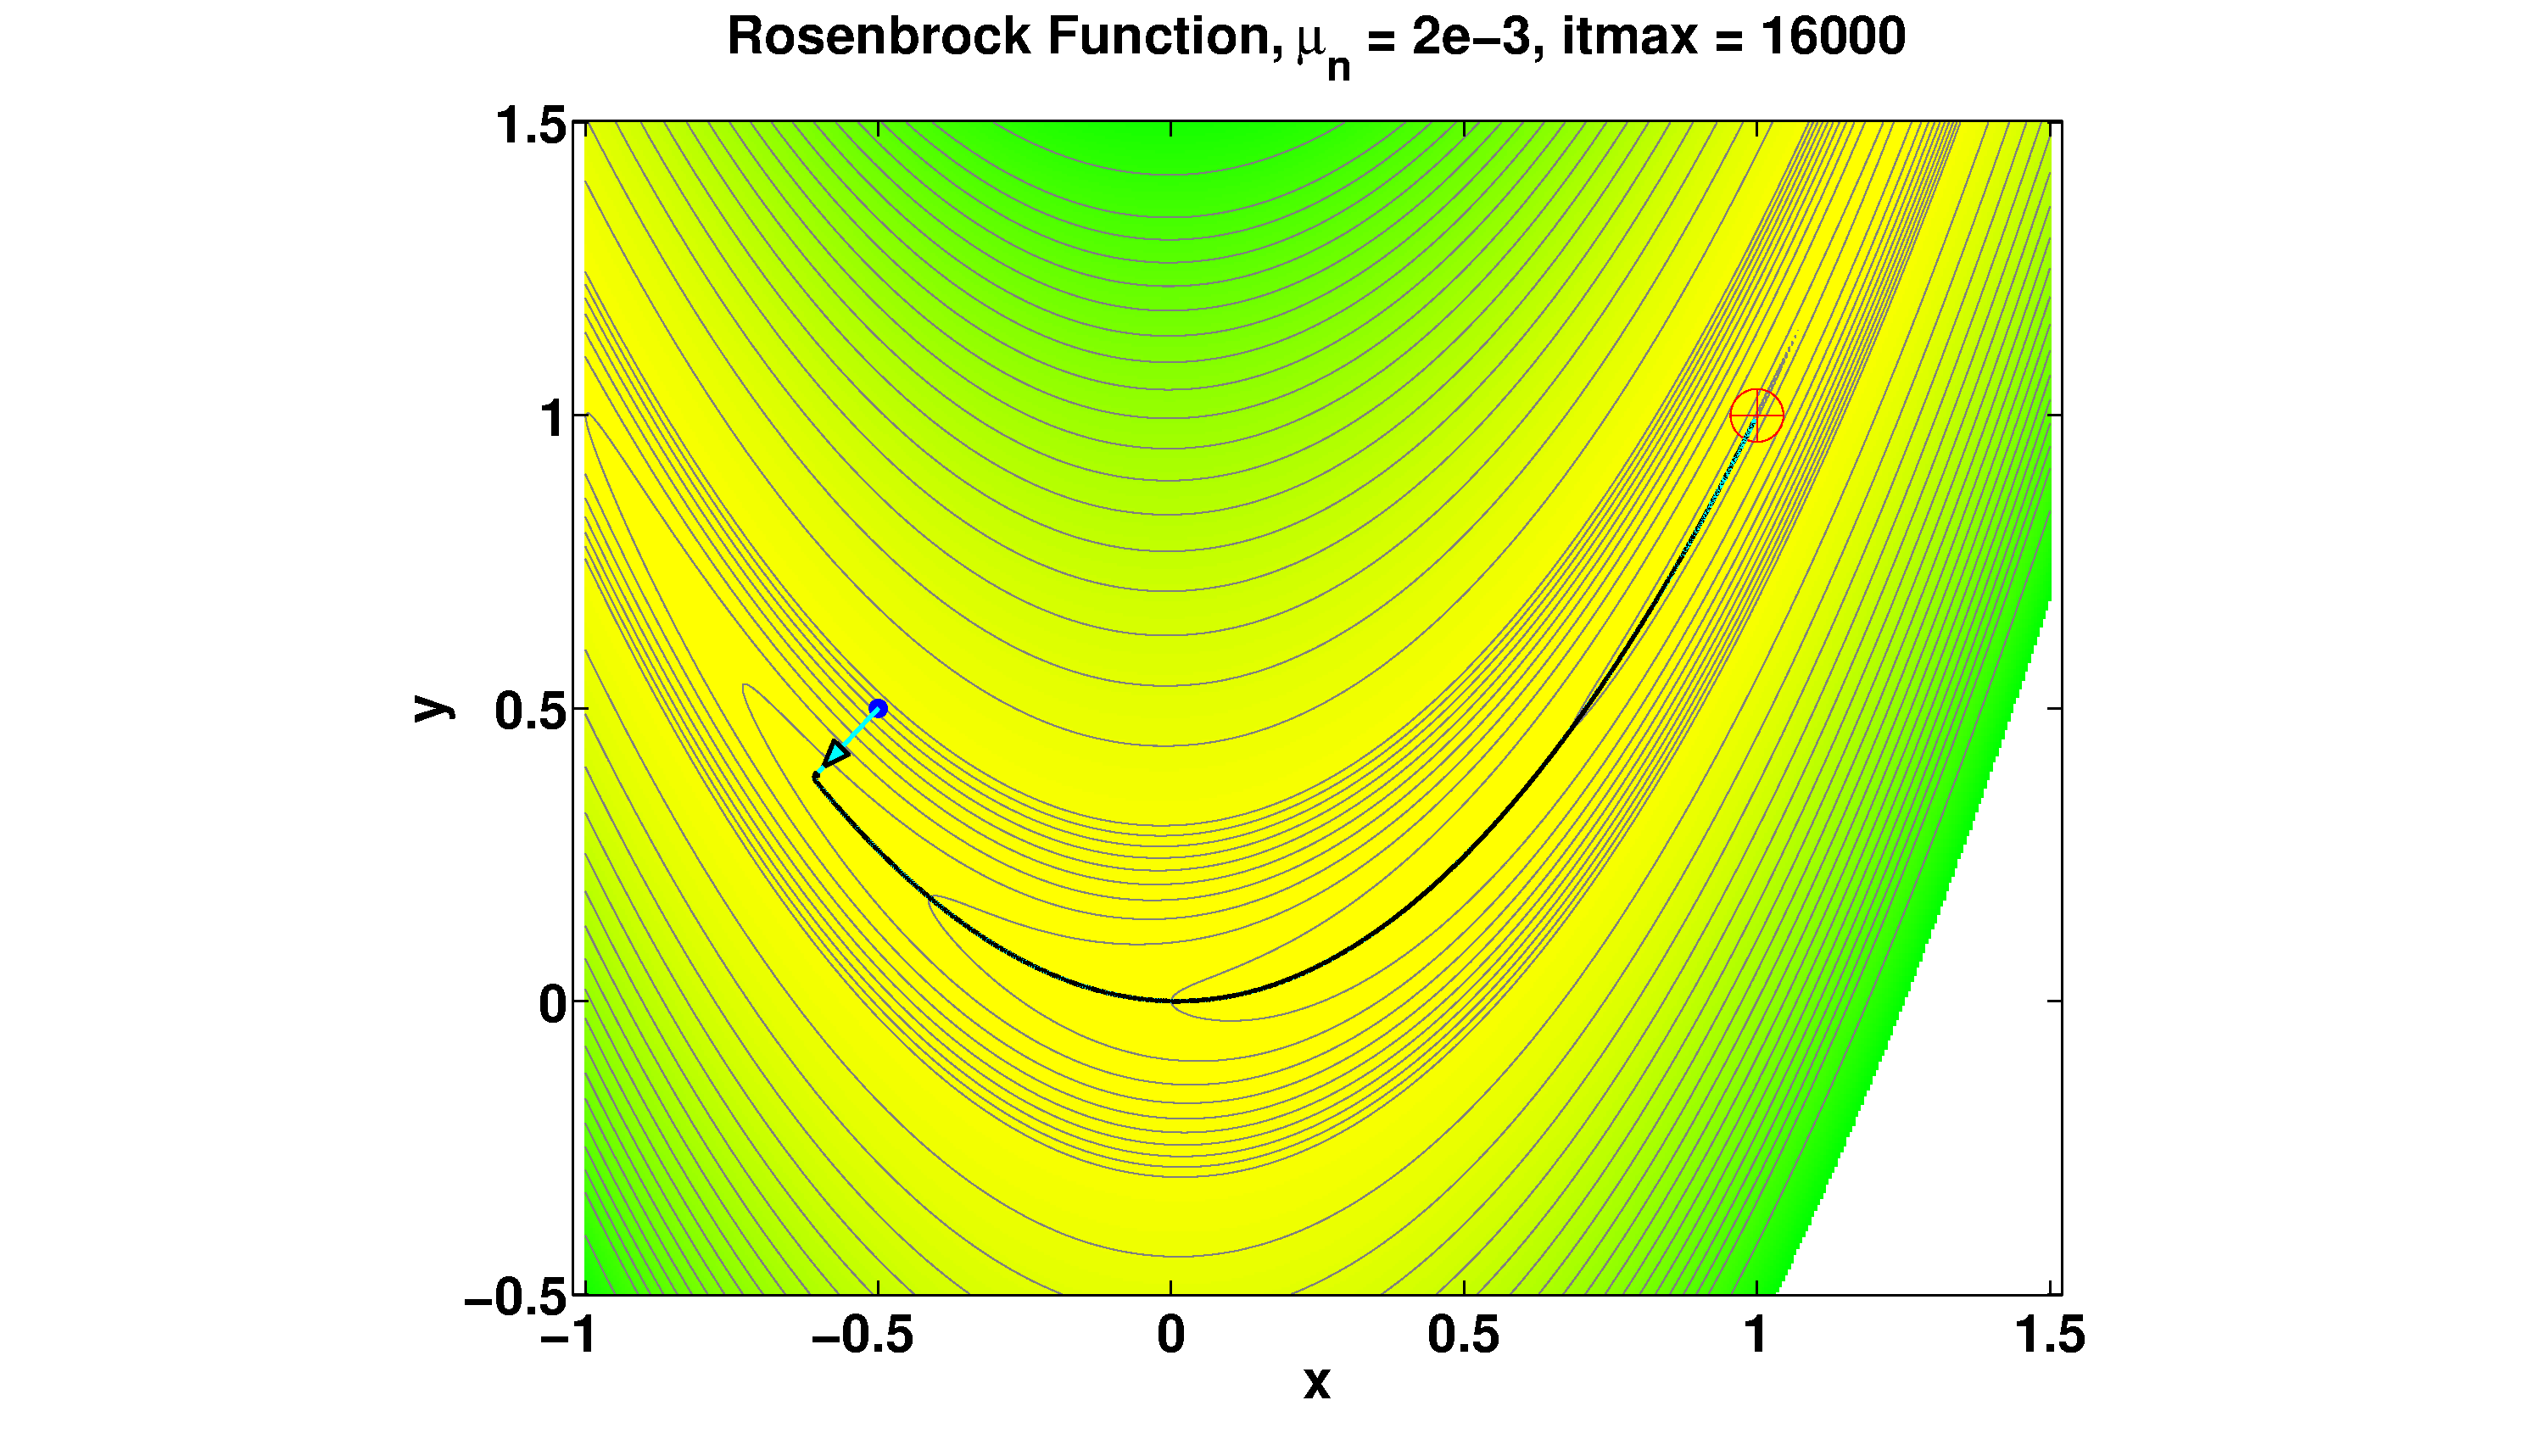
\includegraphics[width=15cm]{figures/Rosenbrock_1.pdf}\\
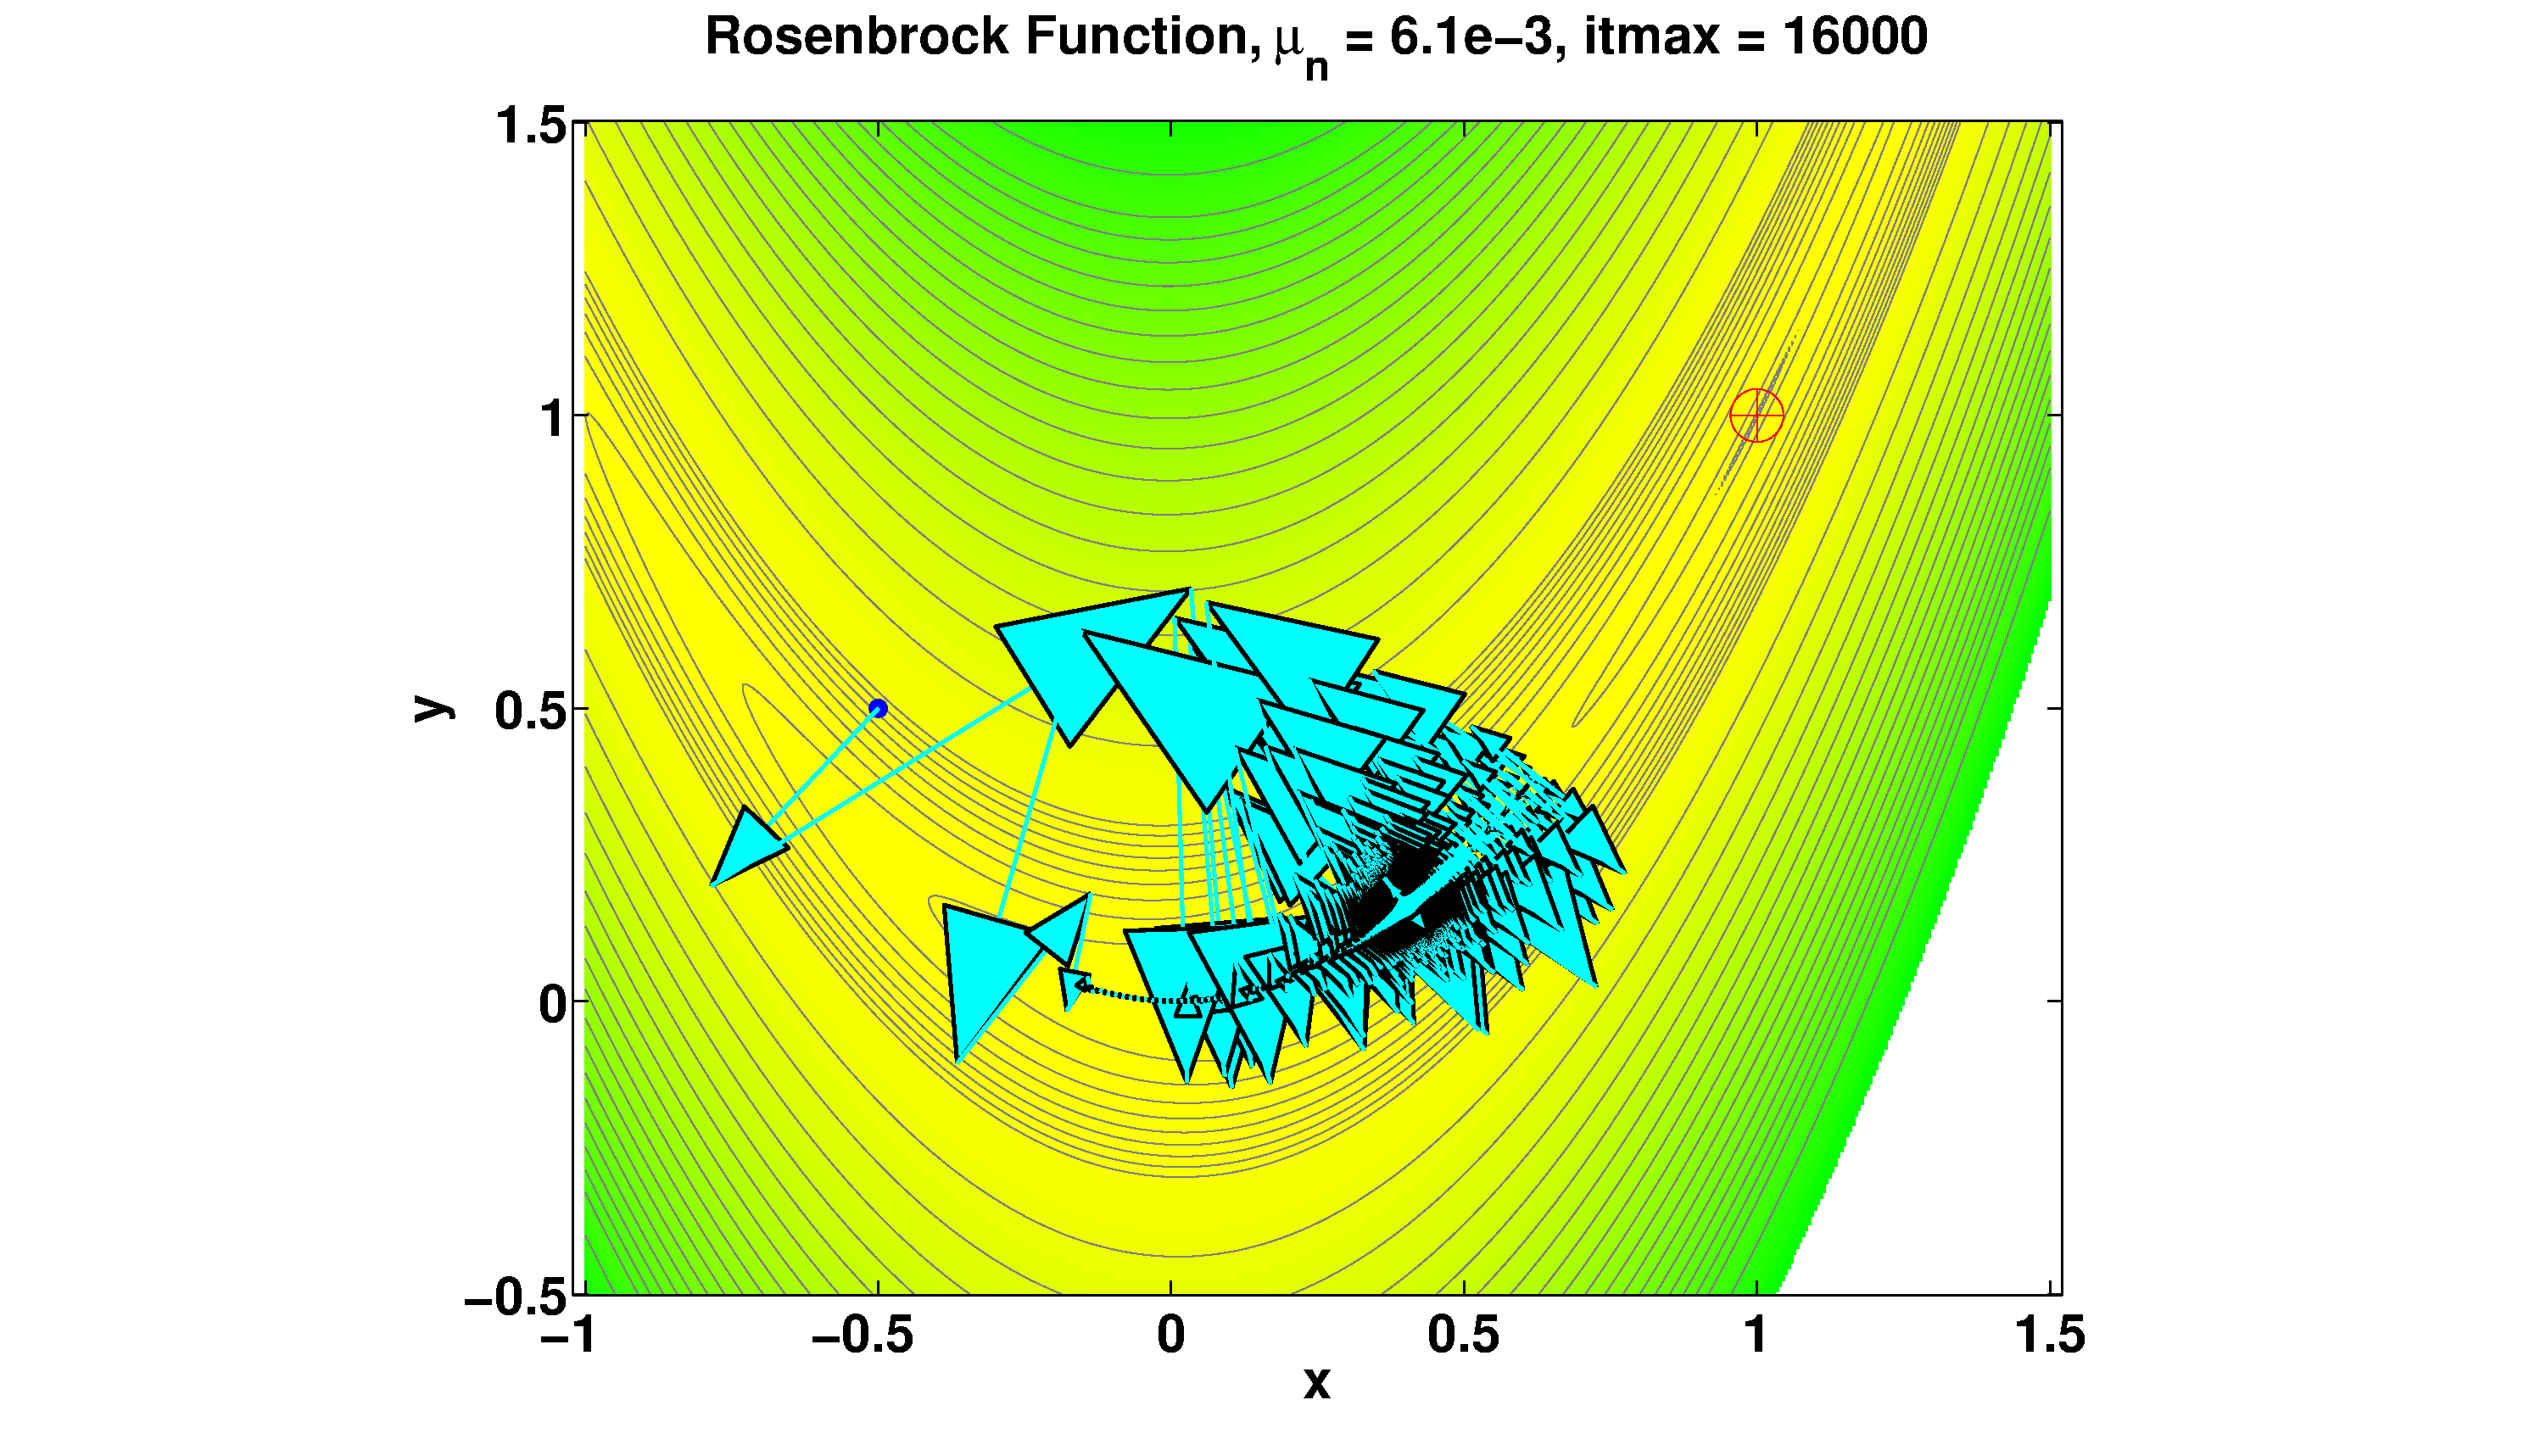
\includegraphics[width=15cm]{figures/Rosenbrock_2.pdf}\\
\caption{Results of the convergence test for the Rosenbrock function. The minimum is marked with a red cross, the starting point with a blue point. The maximum number of iterations is 16000. The step length $\rm{\mu_n}$ varies between $\rm{2e-3}$ (top) and $\rm{6.1e-3}$ (bottom). (\cite{koehn:11})}
\label{Rosenbrock_constant}
\end{center}
\end{figure}
gradient of the Rosenbrock function is large. After reaching the narrow valley the gradient is much smaller and as a result the model updates are also decreasing. This leads to a very slow convergence speed. Especially near the minimum the model updates become very small. When choosing a larger step length ($\rm{\mu_n=2e-3}$, Fig. \ref{Rosenbrock_constant} (bottom)) the model update is larger even when the gradient is small, but the code fails to converge at all. Instead it is trapped in a narrow part of the valley. To solve this problem a variable step length is introduced.
\begin{figure}[ht]
\begin{center}
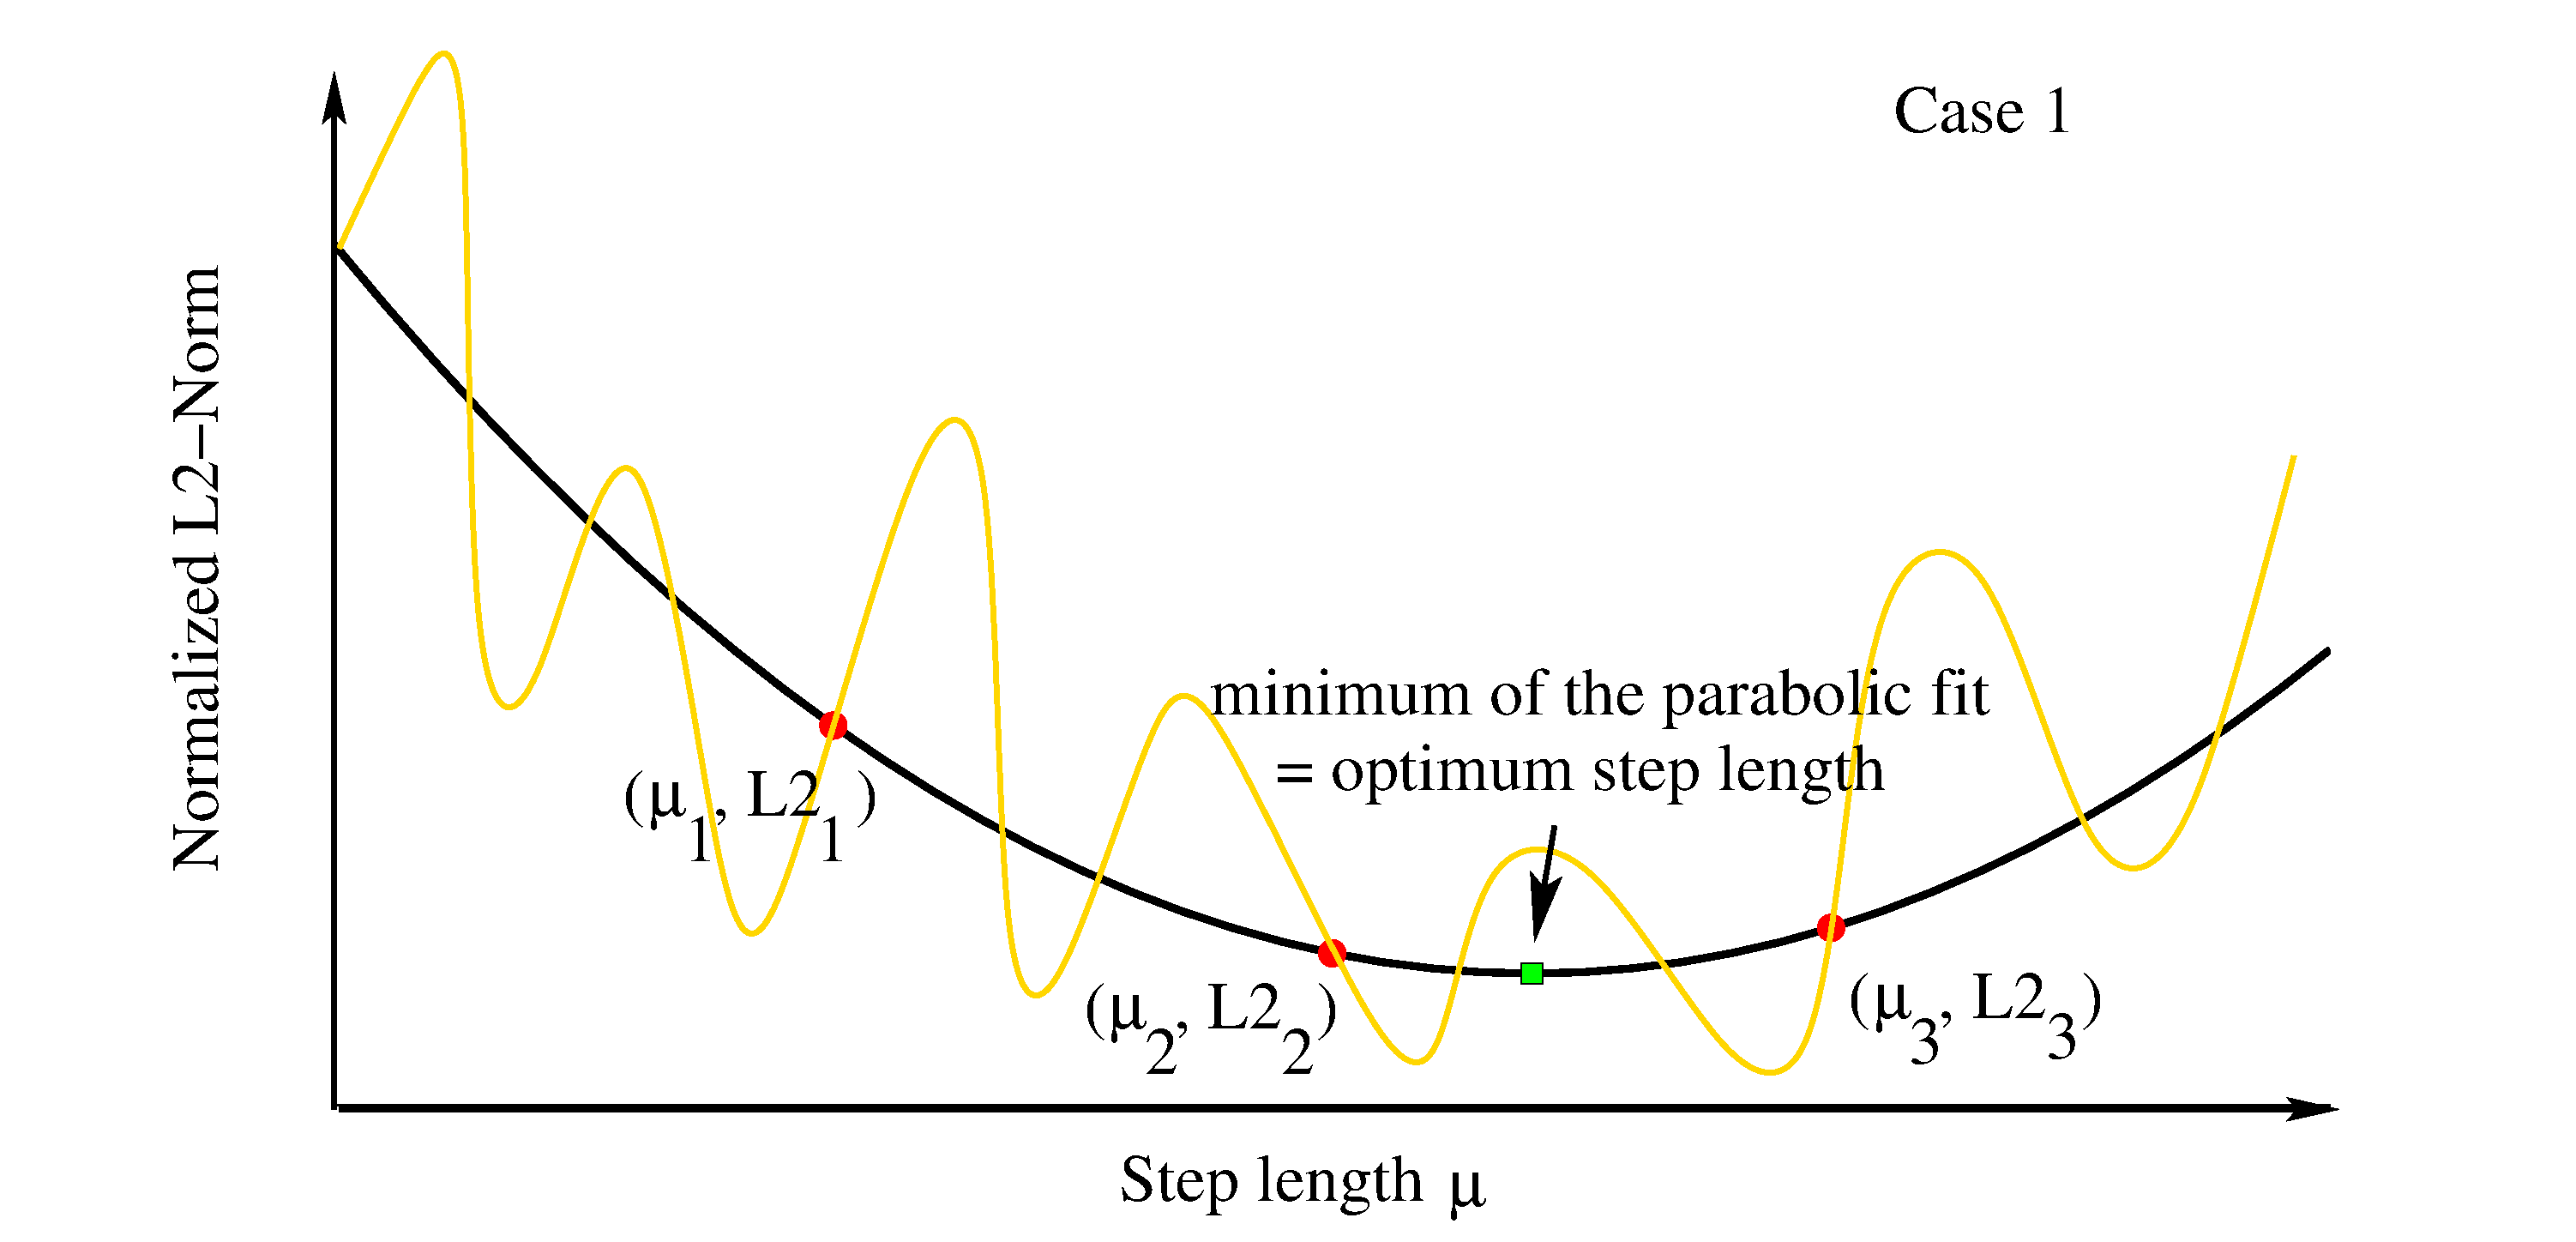
\includegraphics[width=15cm]{figures/sl_case1_final}
\caption{Line search algorithm to find the optimum step length $\rm{\mu_{opt}}$: The true misfit function (yellow line) is approximated by a parabola fitted by 3 points. (\cite{koehn:11})}
\label{sl_case1_final}
\end{center}
\end{figure}
For three test step lengths $\rm{\mu_1}$, $\rm{\mu_2}$ and $\rm{\mu_3}$ three test models are calculated 
\begin{equation}
\begin{split}
\rm{\mathbf{m_{test1}}} &\rm{= \mathbf{m_{n}} + \mu_1 \delta \mathbf{m'_n}}\\
\rm{\mathbf{m_{test2}}} &\rm{= \mathbf{m_{n}} + \mu_2 \delta \mathbf{m'_n}}\\
\rm{\mathbf{m_{test3}}} &\rm{= \mathbf{m_{n}} + \mu_3 \delta \mathbf{m'_n}}\\
\end{split}
\label{parabola1:1}
\end{equation}              
and the corresponding L2-norms $\rm{L2_1}$, $\rm{L2_2}$ and $\rm{L2_3}$ are estimated (Fig. \ref{sl_case1_final}). The true misfit function (yellow line) can be approximated by fitting a parabola through the three points
\begin{equation}
\rm{L2_i = a \mu_i^2 + b \mu_i + c}
\label{parabola}
\end{equation}              
where $\rm{i \in \{1,2,3\}}$ and a, b, c are the unkown coefficients. 
This system of equations can be written as matrix equation:
\EQ{parabola_fit:1}{
\left(
\begin{array}{lll}
\mu_1^2 & \mu_1 & 1\\
\mu_2^2 & \mu_2 & 1\\
\mu_3^2 & \mu_3 & 1\\
\end{array}
\right)\cdot \hspace{0.2 cm}
\left(
\begin{array}{l}
a \\
b \\
c \\
\end{array}
\right)
=
\left(
\begin{array}{l}
L2_1 \\
L2_2 \\
L2_3 \\
\end{array}
\right) \notag
}
or 
\EQ{parabola_fit:2}{\rm{\mathbf{A}\mathbf{x}=\mathbf{b}}.}
The unknown coefficients of this matrix equation are formally defined by
\EQ{parabola_fit:3}{\rm{\mathbf{x}=\mathbf{A}^{-1}\mathbf{b}},}
In the FWT code the solution vector $\rm{\mathbf{x}}$ is calculated by Gaussian elimination. In the following the step length at the extremum of the parabola is defined the extremum step length $\rm{\mu_{ext}}$ (denoted as green square in Fig.\ref{sl_case1_final}). This extremum step length is   
\EQ{parabola_fit:4}{\rm{\mu_{ext}=-\frac{b}{2a}}.}
The application of the variable step length calculation to the Rosenbrock test problem is shown in Fig. \ref{Rosenbrock_variable}. The number of required iteration steps to reach the minimum is reduced by a factor 4 when compared with the constant step length gradient method. The only problem remaining is the slow convergence speed in the small valley of the Rosenbrock function, due to the fact that the update occurs along the gradient direction of the objective function resulting in a ''criss-cross'' pattern. This behaviour can be avoided by applying a nonlinear conjugate gradient method (chapter \ref{NL_Conjugate_Gradient}). In case of the FWT algorithm the three test step lengths for the individual material parameters are calculated by scaling the maximum of the gradient to the maximum of the actual models:
\begin{equation}
\begin{split}
\rm{\mu_\lambda} &= \rm{p \frac{max(\lambda_n)}{max(\delta \lambda_n)}}\\
\rm{\mu_\mu} &= \rm{p \frac{max(\mu_n)}{max(\delta \mu_n)}}\\
\rm{\mu_\rho} &= \rm{p \frac{max(\rho_n)}{max(\delta \rho_n)}}\\
\end{split}
\end{equation}
For most tests in the following chapters $\rm{p_1=0.0025,\;p_2=0.005,\;p_3=0.01}$, which corresponds to maximum model changes of 1/4, 1/2 and 1 \%, worked very well for the optimum step length estimation. All material parameters are updated at the same time. To save computational time the corresponding $\rm{L_2}-$norms are calculated for a few representative shots (in most cases 3). For the acoustic case the step length estimation by parabolic fitting works very well and leads to a smooth decrease of the misfit function during the FWT (Kurzmann (2007), personal communication, \cite{kurzmann:08}). For the multiparameter elastic FWT the misfit function consists of more local minima and therefore the decrease of the objective function is not as smooth as in the acoustic case. \cite{brossier:2009} proposed a more intensive bracketing stage before applying the parabolic fit. For $\rm{p_1=0.0}$ the test step lengths $\rm{p_2}$ and $\rm{p_3}$ are calculated to satisfy the following criteria:
\begin{equation}
\begin{split}
&\rm{L2_2(\mathbf{m_{test2}} = \mathbf{m_{n}} + \mu_2 \delta \mathbf{m'_n}) < L2_1(\mathbf{m_{test1}} = \mathbf{m_{n}})}\\
&\rm{L2_3(\mathbf{m_{test3}} = \mathbf{m_{n}} + \mu_3 \delta \mathbf{m'_n}) > L2_2(\mathbf{m_{test2}} = \mathbf{m_{n}} + \mu_2 \delta \mathbf{m'_n})}\\
\end{split}
\label{parabola1:1:100}
\end{equation}              
This approach leads to a smoother decrease of the objective function, but also increases the number of required forward models.         
\begin{figure}[ht]
\begin{center}
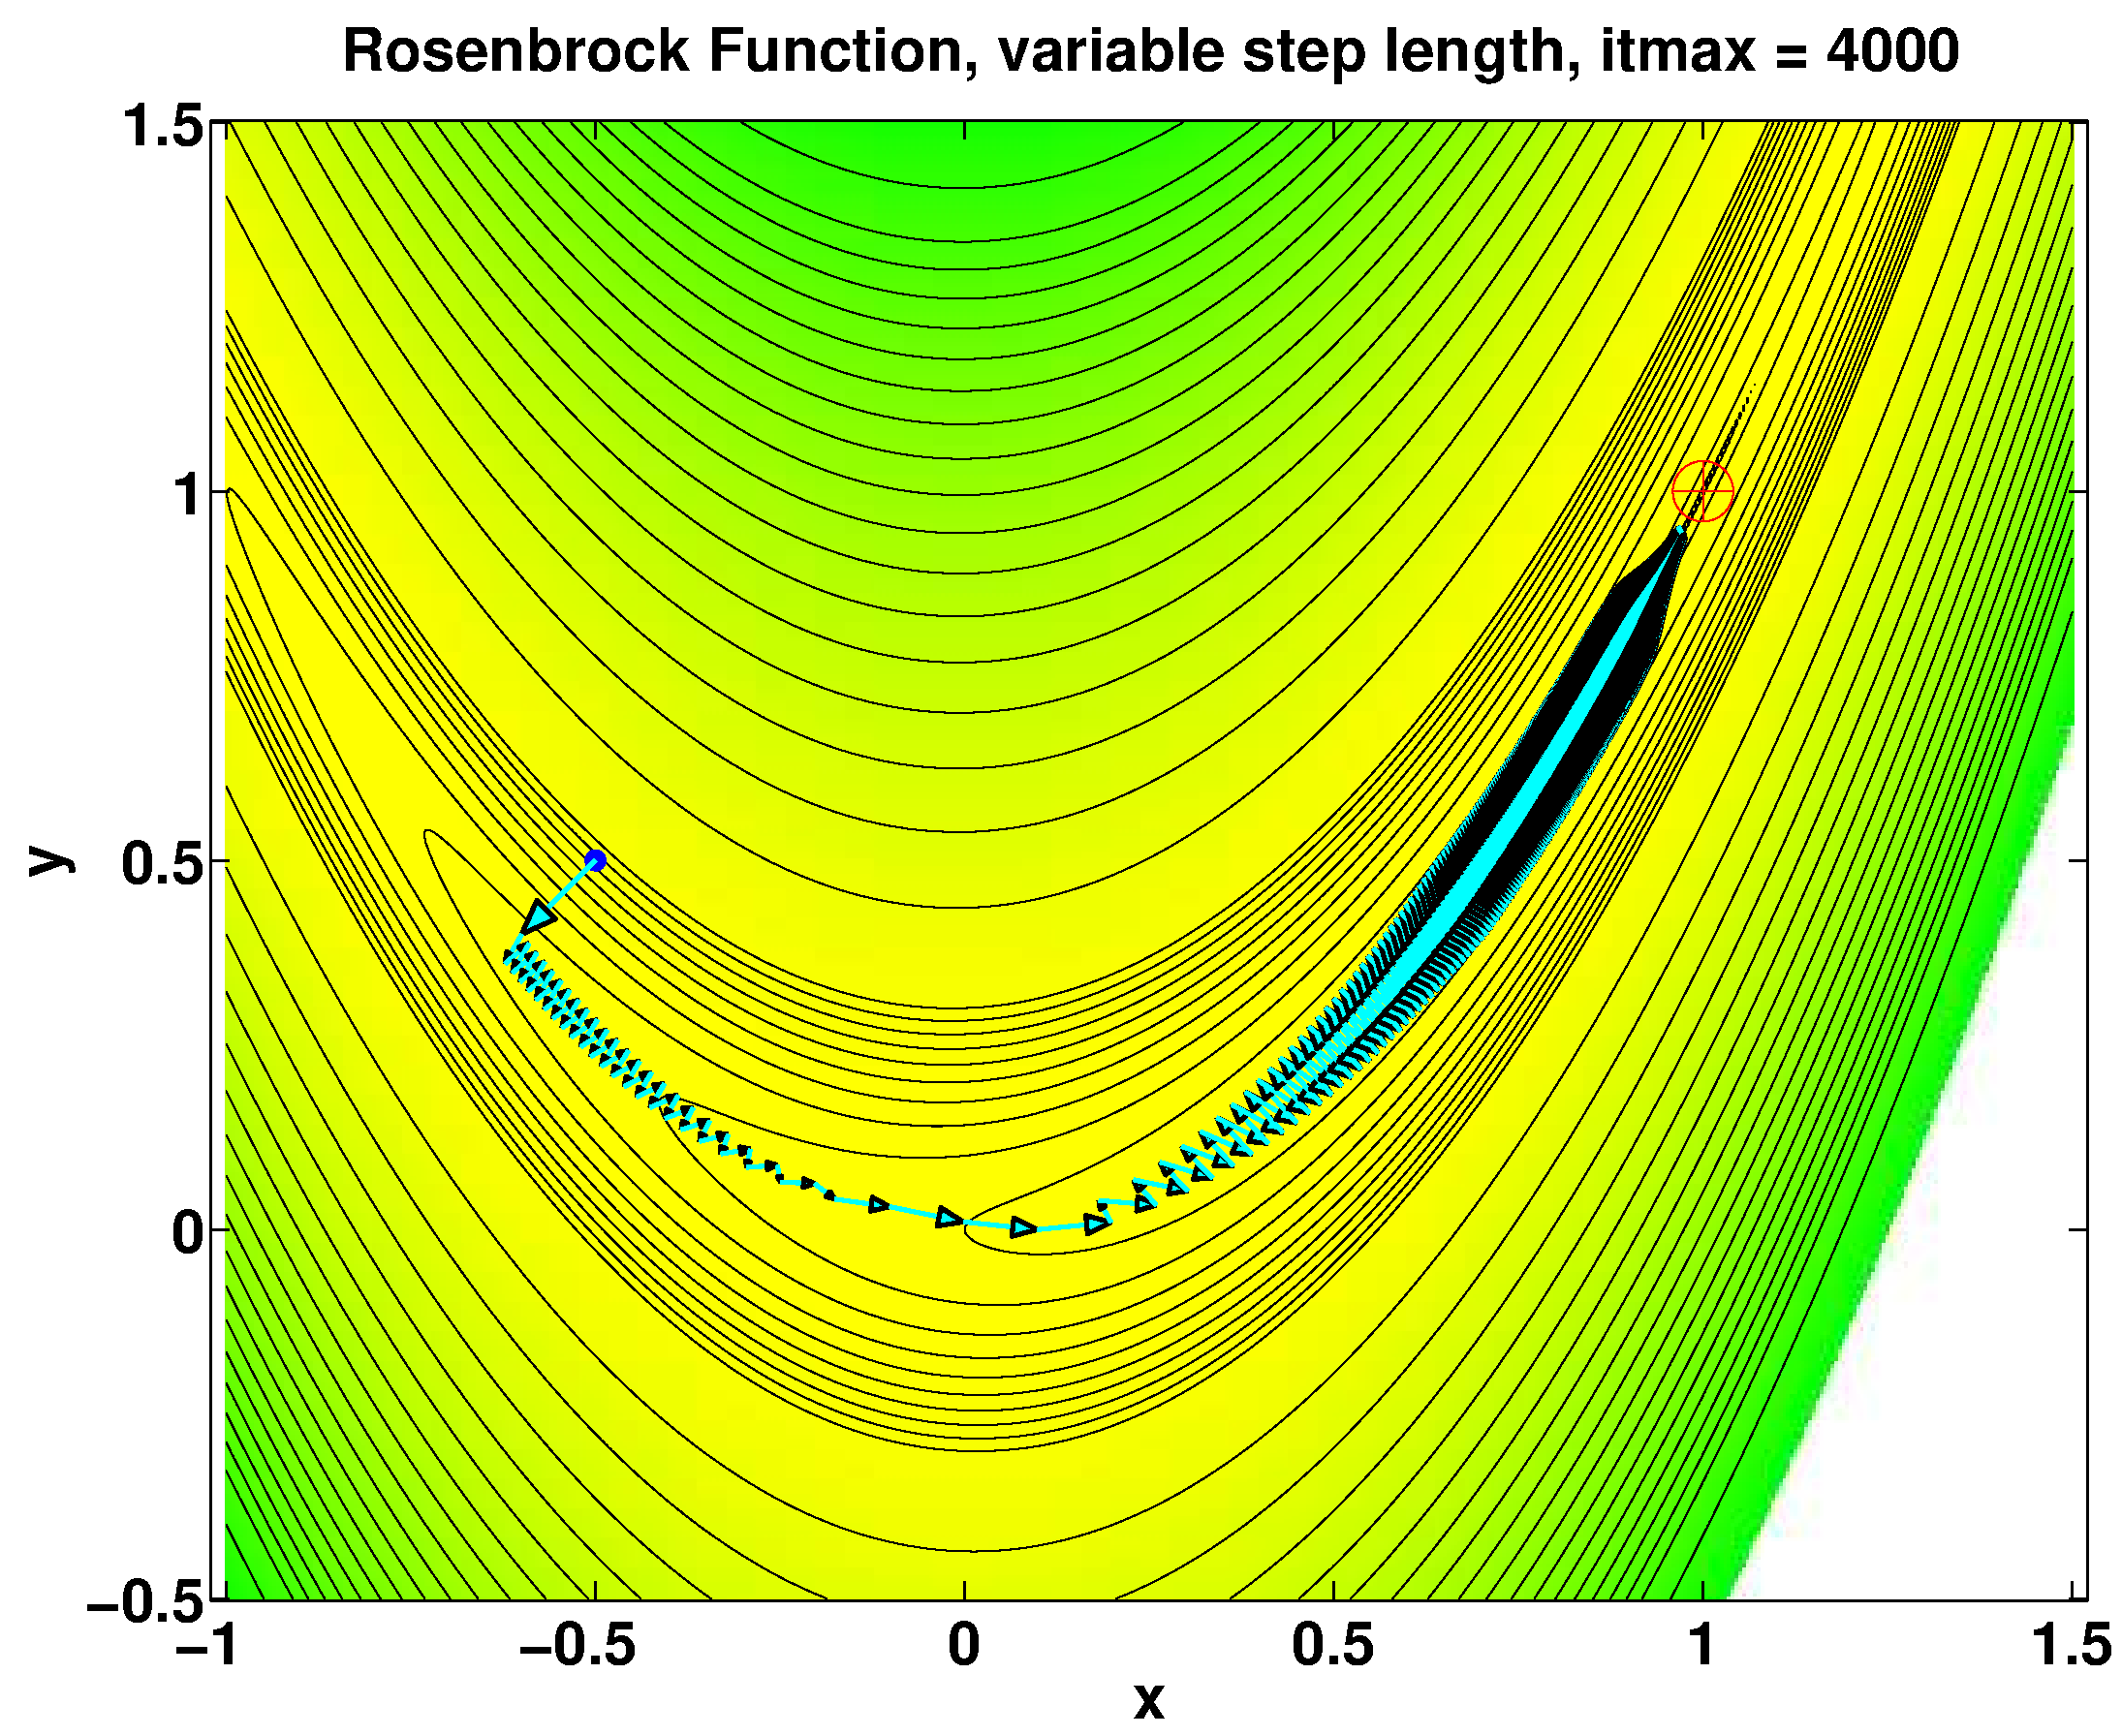
\includegraphics[width=16cm]{figures/Rosenbrock_3}
\caption{Results of the convergence test for the Rosenbrock function. The minimum is marked by a red cross, the starting point by a blue point. The maximum number of iterations is 4000. The optimum step length is calculated at each iteration by the parabola fitting algorithm. Note the criss-cross pattern of the updates in the narrow valley near the minimum. (\cite{koehn:11})}
\label{Rosenbrock_variable}
\end{center}
\end{figure}
\section{Nonlinear Conjugate Gradient Method}\label{NL_Conjugate_Gradient} 
To increase the convergence speed in narrow valleys it would be better to update the model at iteration step n not exactly along the gradient direction $\rm{\delta \mathbf{m}_n}$, but along the conjugate direction $\rm{\delta \mathbf{c}_n}$
\begin{equation}
\rm{\delta \mathbf{c}_n = \delta \mathbf{m}_n + \beta_n \delta \mathbf{c}_{n-1},}  
\label{conj1}
\end{equation}
The first iteration step (n=1) consists of a model update along the steepest descent direction:
\begin{equation} 
\rm{\mathbf{m}_{2} = \mathbf{m}_{1} + \mu_1 \mathbf{\delta m}_{1}, }
\label{conj1:1}
\end{equation}
For all subsequent iteration steps ($\rm{n>1}$) the model is updated along the conjugate direction:
\begin{equation} 
\rm{\mathbf{m}_{n+1} = \mathbf{m}_{n} + \mu_n \mathbf{\delta c}_{n}, }
\label{conj1:2}
\end{equation}
where $ \rm{\delta \mathbf{c}_{1} = \delta \mathbf{m}_1}$.
The weighting factor $\rm{\beta}$ can be calculated in different ways:
\begin{enumerate}
\item Fletcher-Reeves:\\
\begin{equation}
\rm{\beta^{FR}_n=\frac{\delta \mathbf{m}^T_n \delta \mathbf{m}_n}{\delta \mathbf{m}^T_{n-1} \delta \mathbf{m}_{n-1}}}
\label{conj2}
\end{equation}
\item Polak-Ribi$\rm{\acute{e}}$re:\\
\begin{equation}
\rm{\beta^{PR}_n=\frac{\delta \mathbf{m}^T_n (\delta \mathbf{m}_n - \delta \mathbf{m}_{n-1})}{\delta \mathbf{m}^T_{n-1} \delta \mathbf{m}_{n-1}}}
\label{conj3}
\end{equation}
\item Hestenes-Stiefel:\\
\begin{equation}
\rm{\beta^{HS}_n=\frac{\delta \mathbf{m}^T_n (\delta \mathbf{m}_n - \delta \mathbf{m}_{n-1})}{\delta \mathbf{c}^T_{n-1} (\delta \mathbf{m}_n - \delta \mathbf{m}_{n-1})}}
\end{equation}
\end{enumerate}
I use the very popular choice $\rm{\beta_n = max[0,\beta_n^{PR}]}$ which provides an automatic direction reset. This is important because subsequent search directions lose conjugacy requiring the search direction to be reset to the steepest descent direction. Note that the conjugate gradient method doesn't require any additional computational time because only the gradient $\rm{\delta \mathbf{m}_n}$ at two subsequent iterations has to be known. The application of the nonlinear conjugate gradient method combined with the variable step length calculation to the Rosenbrock function is shown in Fig. \ref{Rosenbrock_cg}. The criss-cross pattern of the steepest descent method has vanished. The conjugate gradient method converges already after 2000 iterations compared with 4000 iteration steps of the pure gradient method.   

\begin{figure}[ht]
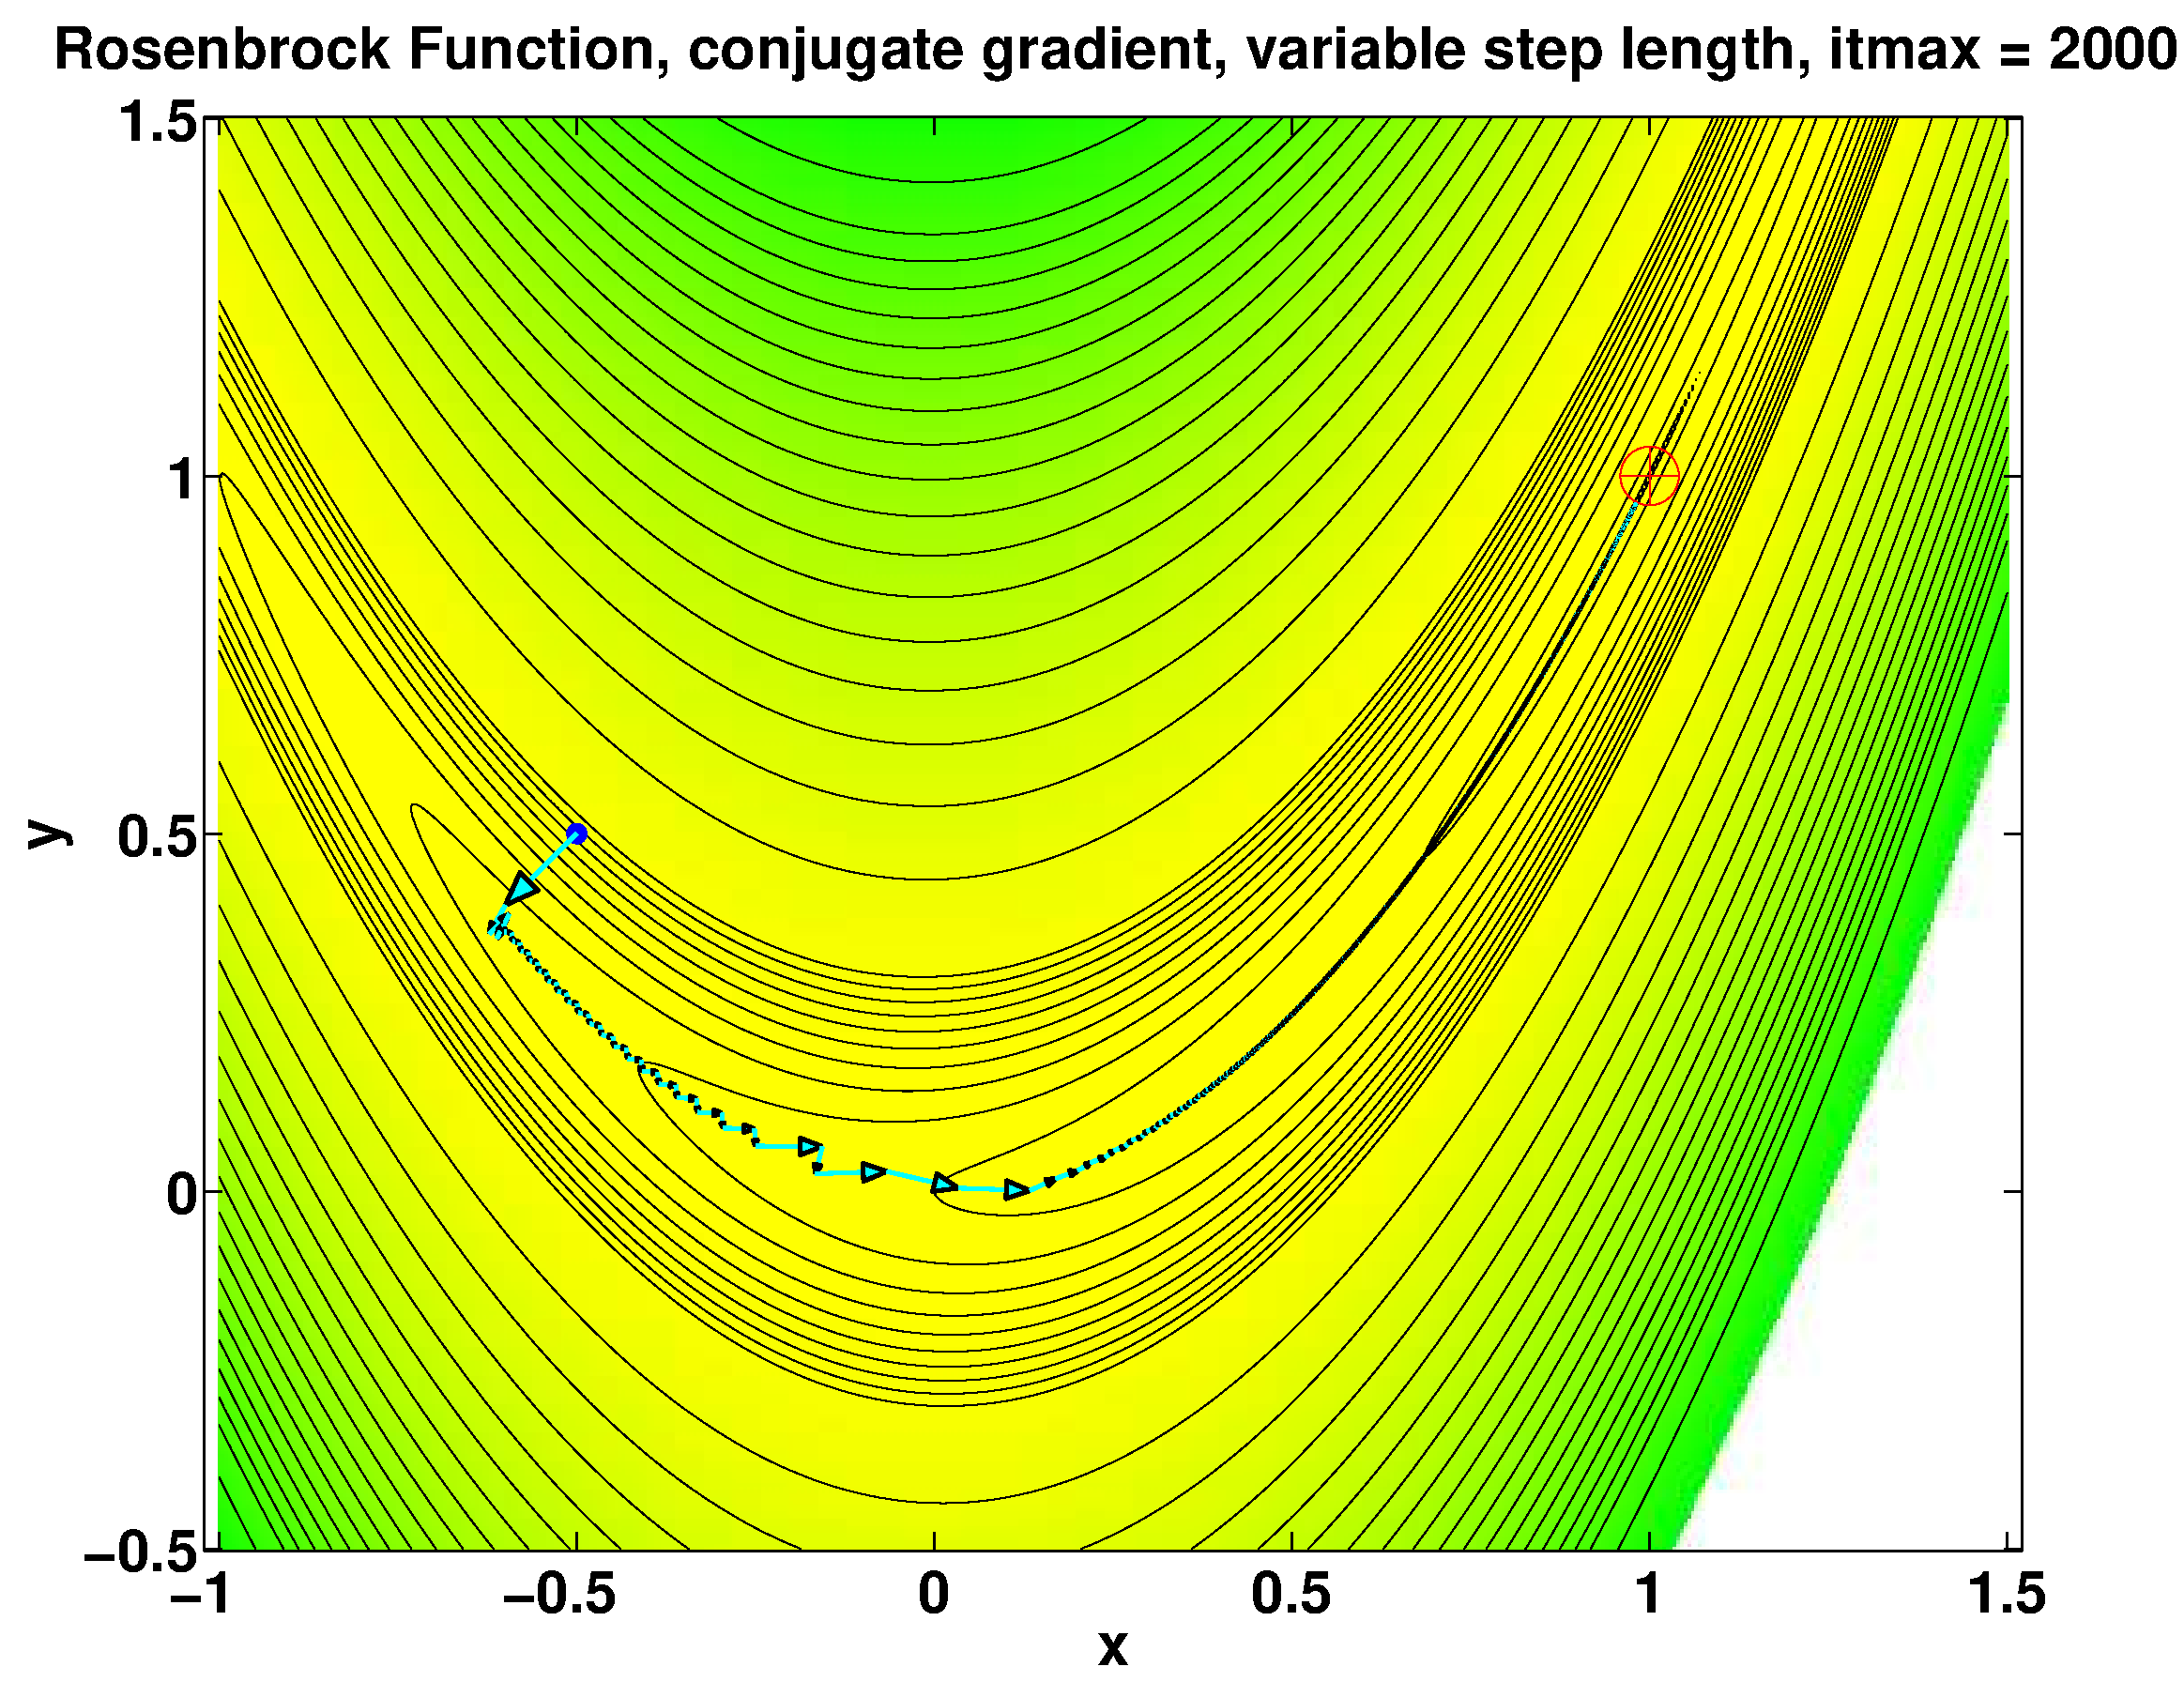
\includegraphics[width=17cm]{figures/Rosenbrock_4}\\
\caption{Results of the convergence test for the Rosenbrock function using the conjugate gradient method, where the optimum step length is calculated with the parabolic fitting algorithm. The minimum is marked by a red cross, the starting point by a blue point. The maximum number of iterations is 2000. (\cite{koehn:11})}
\label{Rosenbrock_cg}
\end{figure}

\clearpage
\section{The elastic FWT algorithm}
In summary the FWT algorithm consists of the following steps:

\begin{enumerate}
\item Define a starting model $\rm{\mathbf{m_1}}$ in the parameter space. This model should represent the long wavelength part of the underground 
very well, because the FWT code is only capable to reconstruct structures at or below the dominant seismic wavelength due to its slow 
convergence speed, the nonlinearity of the problem and the inherent use of the Born approximation to calculate the gradient direction.
\item At iteration step n do:
\begin{enumerate} 
\item For each shot solve the forward problem, stated in Eq.(\ref{2:1}) for the actual model $\rm{\mathbf{m}_n}$ to generate a synthetic dataset 
      $\rm{\mathbf{u^{mod}}}$ and the wavefield $\rm{\mathbf{u}(\mathbf{x},t)}$. 
\item Calculate the residual seismograms $\rm{\delta \mathbf{u} = \mathbf{u^{mod}} - \mathbf{u^{obs}}}$ for the x- and y-components of the
seismic data.
\item Generate the wavefield $\rm{\mathbf{\Psi}(\mathbf{x},t)}$ by backpropagating the residuals from the receiver postions.
\item Calculate the gradients $\rm{\delta \mathbf{m}_n}$ of each material parameter according to Eqs.(\ref{2:28}).
\item To increase the convergence speed an appropriate preconditioning operator P is applied to the gradient $\rm{\delta \mathbf{m}}$
\begin{equation}
\rm{\delta \mathbf{m}^p_n = P \delta \mathbf{m}_n}
\label{2:26:1} 
\end{equation}
Examples of simple preconditioning operator are given in chapter \ref{marmousi_complex_FWT} for a reflection geometry. 
\item For a further increase of the convergence speed calculate the conjugate gradient direction for iteration steps $\rm{n \ge 2}$: 
\begin{equation}
\rm{\delta \mathbf{c}_n = \delta \mathbf{m}^p_n + \beta \delta \mathbf{c}_{n-1}},\; \rm{\text{with}}\; \rm{\delta \mathbf{c}_{1} = \delta
\mathbf{m}^p_1}  
\label{2:26:2}
\end{equation}
where the weighting factor 
\begin{equation}
\rm{\beta^{PR}=\delta \mathbf{m}^p_n \frac{\delta \mathbf{m}^p_n - \delta \mathbf{m}^p_{n-1}}{\delta \mathbf{m}^p_{n-1} \delta \mathbf{m}^p_{n-1}}}
\label{FWT_alg:1}
\end{equation} 
by Polak-Ribi$\rm{\acute{e}}$re is used. The convergence of the Polak-Ribi$\rm{\acute{e}}$re method is guaranteed by choosing 
$\rm{\beta=max[\beta^{PR},0]}$.  
\item Estimate the step length $\rm{\mu_n}$ by the line search algorithm described in chapter \ref{optimum_step_length}.
\item Update the material parameters using the gradient method 
\begin{equation}
\rm{\mathbf{m}_{n+1} = \mathbf{m}_{n} - \mu_n \delta \mathbf{c}_n.}
\end{equation}
If the material parameters are not coupled by empirical relationships it is important to update all three elastic material parameters 
at the same time, otherwise strong artefacts may dominate the inversion result, especially in the case of very complex media.  
\end{enumerate}
\item If the residual energy E is smaller than a given value stop the iteration. Otherwise continue with the next iteration step.  
\end{enumerate}